\documentclass[pdflatex,sn-mathphys-num]{sn-jnl}

%% ================================================================
%% Springer Nature Journal Article Template (sn-jnl Version 3.1)
%% Plant Disease Screening System — Research Paper
%% ================================================================

\usepackage{graphicx}%
\usepackage{multirow}%
\usepackage{amsmath,amssymb,amsfonts}%
\usepackage{amsthm}%
\usepackage[title]{appendix}%
\usepackage{xcolor}%
\usepackage{textcomp}%
\usepackage{manyfoot}%
\usepackage{booktabs}%
\usepackage{algorithm}%
\usepackage{algorithmicx}%
\usepackage{algpseudocode}%
\usepackage{listings}%
\usepackage{array}%
\usepackage{url}%
\usepackage{bookmark}%

\graphicspath{{./}{figures/}}%


\theoremstyle{thmstyleone}%
\newtheorem{theorem}{Theorem}%
\newtheorem{proposition}[theorem]{Proposition}%

\theoremstyle{thmstyletwo}%
\newtheorem{example}{Example}%
\newtheorem{remark}{Remark}%

\theoremstyle{thmstylethree}%
\newtheorem{definition}{Definition}%

\raggedbottom
\vbadness=10000
\vfuzz=30pt
\hbadness=10000
\hfuzz=2pt

\AtBeginDocument{%
  \raggedbottom
  \vbadness=10000
  \hbadness=10000
}

%% ================================================================


\begin{document}

\title[Plant Disease Screening System]{Plant Disease Screening System with MobileNetV3-Small:
Implementation, Exploratory Results, and Validation Gaps}

\author*[1]{\fnm{Mohit} \sur{Sharma}}\email{mohit.12324849@lpu.in}
\author[1]{\fnm{Aniket} \sur{Kumar}}\equalcont{These authors contributed equally to this work.}\email{aniket.12325552@lpu.in}
\author[1]{\fnm{Raghav} \sur{Kumar}}\equalcont{These authors contributed equally to this work.}\email{raghavmumar23@lpu.in}

\affil*[1]{\orgdiv{Department of Computer Science and Engineering},
  \orgname{Lovely Professional University},
  \orgaddress{\city{Phagwara}, \state{Punjab}, \postcode{144411}, \country{India}}}

\abstract{
Plant diseases cause between 20\% and 40\% of global crop yield losses annually, imposing
severe threats to food security where smallholder farmers lack timely diagnostic expertise \citep{savary2019burden}.
This paper presents a comprehensive implementation, empirical evaluation, and full-stack CPU deployment of a
plant disease screening system built upon lightweight convolutional neural networks. Models are trained on a
curated combined corpus of 56{,}433 images across 38 classes (40{,}151 training [37{,}992 PlantVillage + 2{,}159 PlantDoc],
5{,}436 validation, 5{,}429 calibration, and 5{,}417 holdout test images, constructed after rigorous deduplication and
leakage exclusion). Four architectures are systematically benchmarked under an identical protocol: 3 total completed epochs
(1 head warmup epoch with frozen backbone at lr $10^{-3}$, followed by 2 fine-tuning epochs at backbone lr $10^{-5}$ and
head lr $10^{-4}$ with CosineAnnealingLR), batch size 8, AdamW, and label smoothing 0.10. On the reserved PlantVillage holdout
test partition (5{,}417 images), MobileNetV3-Large achieves 95.96\% top-1 accuracy (Macro-F1 94.52\%), while MobileNetV3-Small
provides optimal computational efficiency with 95.02\% top-1 accuracy (Macro-F1 93.13\%), 9.42\,ms CPU forward latency,
and a 6.06\,MB disk footprint. External evaluation on 236 natural-background PlantDoc images reveals a severe domain shift
of approximately 56 percentage points (MobileNetV3-Small top-1: 38.98\%, top-3: 64.83\%, Macro-F1 across 27 represented ground-truth
classes: 36.84\%, Macro-F1 across 32 observed classes: 31.08\%, Macro-F1 across the full 38-class taxonomy: 26.17\%, and Weighted-F1: 37.41\%).
An assistive multi-scale sliding-window candidate-region screening pipeline evaluated against 452 ground-truth leaf bounding boxes achieves
38.05\% localization recall at IoU~$\geq~0.25$ with 844.25\,ms latency, more than doubling baseline recall (18.14\%).
To support practical usage, the system is integrated into a complete CPU-optimized FastAPI backend and React frontend
utilizing a verified Phase 5 MobileNetV3-Small TorchScript export (SHA-256: \texttt{6fff52f1...}). The deployed application
decouples whole-leaf classification from candidate-region screening, enforces uncalibrated inference ($T=1.0$) with an
operational review threshold of 0.60, and visualizes exploratory Grad-CAM saliency. Robustness stress tests across 20 synthetic
perturbations reveal key vulnerabilities, notably severe overexposure where disease textures wash out and flip diseased leaves to
healthy (at 63.79\% confidence), evading the review threshold. Critical validation gaps, domain shift bounds, and non-autonomous
triage protocols are documented to provide a rigorous, reproducible foundation for field-deployable agricultural AI.
}

\keywords{Plant disease detection, Deep learning, MobileNetV3, Domain generalization, Candidate-region screening, Temperature calibration}

\maketitle

%% ================================================================
%% 1. INTRODUCTION
%% ================================================================

\section{Introduction}
\label{sec:introduction}

Agricultural crop losses attributable to fungal, bacterial, and viral plant diseases
represent one of the most pressing threats to global food security. \citet{savary2019burden}
estimated that pathogens and pests collectively reduce yields of the world's five major
staple crops---wheat, rice, maize, potato, and soybean---by 10\%–40\% annually. In many
low- and middle-income countries, smallholder farmers who cultivate the majority of food
are disproportionately impacted because they typically have limited access to plant
pathology expertise, agrochemical advisory services, or digital tools for timely disease
identification.

Computer vision and deep learning have emerged as promising technologies to democratise
plant disease diagnosis. The seminal work of \citet{mohanty2016} demonstrated that deep
convolutional neural networks (CNNs) could classify 26 diseases across 14 crop species
at over 99\% accuracy under controlled PlantVillage \citep{hughes2015plantvillage}
laboratory conditions. Subsequent work consistently replicated high in-domain accuracy
\citep{ferentinos2018deep,chen2020identification,atila2021plant}, fuelling optimism about
AI-driven agricultural diagnostics.

However, three critical gaps separate laboratory benchmarks from reliable field
deployment.

First, \textit{domain shift}: models trained exclusively on PlantVillage images---where
individual leaves are photographed against plain grey or black backgrounds---perform
substantially worse on natural photographs with complex backgrounds, variable lighting,
multi-leaf occlusion, and camera motion blur \citep{barbedo2016review,singh2020plant,dsouza2023generalization}.
\citet{toda2019deep} and \citet{thapa2020plant} confirmed that apparent accuracy improvements
on curated benchmarks frequently fail to transfer to in-field conditions.

Second, \textit{probability calibration}: modern CNNs are often overconfident or
underconfident in their predicted probabilities, limiting the utility of confidence
thresholds for autonomous field decision-making or agricultural expert review \citep{guo2017calibration,minderer2021calibration}.
Without calibration, a model reporting 95\% confidence cannot be trusted to be correct
95\% of the time.

Third, \textit{whole-plant localization}: practical field photographs typically contain
multiple leaves, background vegetation, soil, and sky. Classifying the entire image as a
single class conflates contributions from healthy and diseased plant material
\citep{barbedo2018factors,ren2015fasterrcnn}.

This paper addresses all three gaps through a systematic, multi-phase experimental
programme. The contributions are:

\begin{enumerate}
  \item A reproducible dataset pipeline with duplicate-aware splitting, SHA-256 manifest
        verification, and strict partition isolation across training, validation,
        calibration, and holdout test sets.
  \item A comparative benchmark of four lightweight CNN architectures (MobileNetV3-Small,
        MobileNetV3-Large, EfficientNet-B0, and ResNet18) evaluated under
        identical protocols on CPU hardware.
  \item Post-hoc temperature scaling calibration applied separately for each architecture
        using an isolated calibration partition, with pre- and post-calibration Expected
        Calibration Error (ECE) reported transparently.
  \item An independent external evaluation on 236 PlantDoc natural-background images,
        quantifying the domain gap without fine-tuning or threshold adaptation.
  \item A candidate-region screening pipeline using multi-scale sliding windows, Excess
        Green Index (ExG) foliar saliency filtering, 12\% context padding, and hybrid
        NMS, evaluated against 452 whole-leaf bounding-box annotations.
\end{enumerate}

\subsection{Research Gap}
\label{sec:research_gap}

A specific gap motivating this work was identified in prior exploratory research on the
same system: the initial MobileNetV3-Small checkpoint lacked verifiable training-split
provenance, the external PlantDoc evaluation had not been conducted, the calibrated
temperature parameter used offline differed from the application configuration, and no
multi-architecture comparison existed. This paper directly addresses each of these gaps
using completed experimental evidence from a structured five-phase research programme.

\subsection{Research Objectives}
\label{sec:objectives}

The primary objectives of this study are:
\begin{enumerate}[(i)]
  \item To establish a fully reproducible training protocol with cryptographic checkpoint
        provenance for all evaluated architectures.
  \item To quantify the classification performance of four lightweight CNN architectures
        on the controlled PlantVillage holdout test set.
  \item To evaluate cross-domain generalization on external, unconstrained PlantDoc images.
  \item To apply and evaluate post-hoc temperature scaling calibration for each architecture.
  \item To design, implement, and evaluate a multi-scale candidate-region screening
        pipeline for whole-plant field images.
  \item To identify and transparently document remaining performance gaps and
        architectural limitations.
\end{enumerate}

%% ================================================================
%% 2. LITERATURE REVIEW
%% ================================================================

\section{Literature Review}
\label{sec:literature_review}

\subsection{Deep Learning Architectures for Edge Foliar Diagnosis}
The field of automated plant pathology advanced rapidly following \citet{mohanty2016}, who demonstrated near-human classification accuracy on the PlantVillage corpus. Subsequent studies employing AlexNet, VGG, Inception, and ResNet architectures consistently confirmed top-1 accuracies exceeding 95\% under uniform laboratory imaging \citep{ferentinos2018deep,too2019comparative,kamilaris2018deep}. However, deploying deep models on resource-constrained agricultural edge devices necessitates lightweight parameter footprints \citep{howard2017mobilenets}. The MobileNet family introduces depthwise separable convolutions, cutting inference FLOPs by nearly an order of magnitude relative to standard convolutions. MobileNetV3 \citep{howard2019mobilenetv3} further incorporates Neural Architecture Search (NAS), Squeeze-and-Excitation (SE) attention \citep{hu2018squeeze}, and hard-swish non-linearities to maximize mobile efficiency. Complementary lightweight paradigms include EfficientNet-B0 \citep{tan2019efficientnet}, which balances network depth, width, and input resolution via compound scaling, and ResNet-18 \citep{he2016resnet}, which leverages residual shortcuts as an enduring, well-characterized baseline \citep{atila2021plant}.

\subsection{Laboratory Benchmarks and the Natural Field Domain Shift}
PlantVillage \citep{hughes2015plantvillage} remains the foundational foliar benchmark, comprising 54{,}305 laboratory images across 38 crop classes. Nonetheless, its ecological validity has been extensively critiqued \citep{barbedo2016review,toda2019deep,dsouza2023generalization}, as models trained solely on uniform backgrounds exploit spurious context cues that fail in open field environments. To evaluate in-the-wild transfer, PlantDoc \citep{singh2020plant} introduced 2{,}598 natural-background images across 27 plant disease categories. Evaluations on PlantDoc consistently reveal severe accuracy degradations of 30\%--60\% relative to PlantVillage. Mitigations including extensive geometric augmentation \citep{shorten2019survey}, domain adaptation, and mixed-corpus fine-tuning \citep{kwak2023effect} alleviate but do not close this generalization bound. Furthermore, \citet{toda2019deep} used Grad-CAM visualisations \citep{selvaraju2017gradcam} to show that CNN representations degrade when natural foliage noise fractures foliar feature maps.

\subsection{Probabilistic Calibration and Assistive Screening Localization}
Modern deep neural networks are prone to systematic overconfidence, predicting near-unity probabilities on incorrect or out-of-distribution inputs \citep{guo2017calibration}. Post-hoc temperature scaling offers a computationally lightweight parametric solution, rescaling pre-softmax logits via an optimized scalar $T > 0$ to minimize Expected Calibration Error (ECE) \citep{niculescu2005calibration,minderer2021calibration}. Moreover, because whole-image classification fails on multi-leaf or canopy photographs, localized screening approaches are essential. While dense object detectors such as Faster R-CNN \citep{ren2015fasterrcnn} and YOLO \citep{redmon2016yolo} demand exhaustive bounding-box training annotations, class-agnostic candidate-region proposals combined with foliar color indices (e.g., Excess Green, ExG) \citep{woebbecke1995color} enable efficient assistive leaf screening using pre-trained classifiers \citep{jiang2019realtime,he2021multiscale}.

%% ================================================================
%% 3. METHODOLOGY
%% ================================================================

\section{Methodology}
\label{sec:methodology}

\subsection{Dataset Composition and Partitioning}
\label{sec:dataset}

\subsubsection{Source Datasets}

Two public datasets were combined:
\begin{itemize}
  \item \textbf{PlantVillage} \citep{hughes2015plantvillage}: 54{,}305 images across
        38 plant disease and health categories, photographed against controlled uniform
        backgrounds. All images were collected from the official colour-image archive.
  \item \textbf{PlantDoc} \citep{singh2020plant}: 2{,}598 training images and 236 test
        images collected from real-world photographs with complex natural backgrounds.
        The classification test set (236 images) is treated as an independent external
        benchmark and is never used for training, validation, or parameter tuning.
        The object-detection annotations (452 whole-leaf bounding boxes across 236 test
        images) are used exclusively for candidate-region screening evaluation.
\end{itemize}

\subsubsection{Duplicate Removal}

A global perceptual hash deduplication audit was conducted across all 54{,}305
PlantVillage images. The audit identified:
\begin{itemize}
  \item \textbf{10 cross-label exact duplicates}: Identical images appearing under two
        or more conflicting disease labels (e.g.\ the same leaf assigned to both
        \textit{Orange Huanglongbing} and \textit{Peach Bacterial Spot}) were removed
        from the split manifest to eliminate contradictory gradient updates.
  \item \textbf{21 intra-class exact duplicates}: Identical image pairs within the same
        disease class were removed to prevent pseudo-replication and cross-split leakage.
\end{itemize}

Additionally, deduplication between PlantDoc training and test sets eliminated benchmark contamination. An exploratory file-level audit between the raw \texttt{train/} and \texttt{test/} directories identified 10 duplicate image pairs sharing identical cryptographic hashes. However, one of these images was simultaneously an intra-training duplicate of another training image. Consequently, during formal programmatic manifest construction, that redundant image was accounted for under intra-training deduplication, leaving exactly 9 unique test-duplicate image records and 4 near-duplicate perceptual pairs removed specifically under test-leakage exclusion rules.

\subsubsection{Partition Isolation}

The cleaned PlantVillage corpus (54{,}274 images) was partitioned using stratified
random sampling with seed 42 into four non-overlapping partitions:

\begin{table}[htbp]
\caption{Dataset partitions used in this study. Each partition is fully isolated with no sample overlap. The combined split manifest comprises 56{,}433 records (37{,}992 PlantVillage training images, 2{,}159 PlantDoc training images, 5{,}436 PlantVillage validation images, 5{,}429 PlantVillage calibration images, and 5{,}417 PlantVillage holdout test images). The official external PlantDoc test benchmark (236 images, 452 ground-truth whole-leaf annotations) is strictly held out and was never observed during gradient updates, architecture selection, or hyperparameter tuning.}\label{tab:dataset_partitions}%
\footnotesize
\setlength{\tabcolsep}{2.5pt}%
\begin{tabular*}{\textwidth}{@{\extracolsep\fill}>{\raggedright\arraybackslash}p{2.2cm}>{\raggedright\arraybackslash}p{3.2cm}rr>{\raggedright\arraybackslash}p{3.2cm}}
\toprule
\textbf{Partition} & \textbf{Source Dataset \& Rule} & \textbf{Images} & \textbf{Classes} & \textbf{Operational Role} \\
\midrule
Training Split & PlantVillage (37{,}992) + PlantDoc Train (2{,}159) & 40{,}151 & 38 & Gradient updates only \\
Validation Split & PlantVillage Holdout Slice (disjoint) & 5{,}436 & 38 & Model selection \& early stop \\
Calibration Split & PlantVillage Holdout Slice (disjoint) & 5{,}429 & 38 & Temperature calibration \\
Holdout Test Split & PlantVillage Holdout Slice (disjoint) & 5{,}417 & 38 & In-domain evaluation \\
\midrule
\textbf{Combined Manifest} & \textbf{Deduplicated Multi-Source Corpus} & \textbf{56{,}433} & \textbf{38} & \textbf{SHA-256: \texttt{f9ef8b9d...}} \\
\midrule
External PlantDoc & Official Test Benchmark (natural field) & 236 & 27 & OOD domain evaluation \\
PlantDoc Leaves & Bounding-box annotations on test images & 452 & 27 & Candidate screening eval \\
\botrule
\end{tabular*}
\end{table}

\noindent\textit{Data Provenance and Exact PlantDoc Funnel Reconciliation}:
The progression from raw external source downloads to the final training and evaluation partitions is governed by strict, documented exclusion rules:
\begin{enumerate}
  \item \textbf{Raw Repository Downloads (2{,}598 images)}: The upstream PlantDoc repository \citep{singh2020plant} contains 2{,}598 total image files.
  \item \textbf{File Integrity Audit (256 exclusions $\rightarrow$ 2{,}342 images)}: Initial decoding identified 256 unreadable, empty (0-byte), or severely corrupted image files that failed standard PIL/OpenCV loading, establishing an audited pool of 2{,}342 readable classification images.
  \item \textbf{Documented Training Exclusions (183 exclusions $\rightarrow$ 2{,}159 images)}: Before incorporating PlantDoc images into the combined training corpus, systematic deduplication and leakage auditing identified 183 exclusions:
  \begin{itemize}
    \item \textit{Corrupt or Missing Records}: 117 image records with unresolvable paths or truncated data (\texttt{plantdoc\_corrupt\_or\_missing}).
    \item \textit{Intra-Training Duplicates}: 53 redundant image instances within the PlantDoc training partition (\texttt{plantdoc\_duplicate\_within\_training}).
    \item \textit{Exact Test Duplicates}: 9 unique image records sharing identical SHA-256 hashes with images in the official 236-image PlantDoc test benchmark (\texttt{plantdoc\_duplicate\_of\_plantdoc\_test}). Note that while an initial directory comparison identified 10 duplicate pairs, one image was an internal training duplicate already captured under the 53 intra-training exclusions; thus, exactly 9 unique test-matching records were removed here.
    \item \textit{Near-Duplicate Test Leakage}: 4 image records identified via perceptual hashing as near-duplicate pairs of official test images (\texttt{plantdoc\_near\_duplicate\_of\_plantdoc\_test}).
  \end{itemize}
  Subtracting these 183 documented exclusions ( + 53 + 9 + 4 = 183$) from the 2{,}342 audited images yields exactly {,}159$ clean, non-leaking training images.
  \item \textbf{Combined Split Manifest (56{,}433 total records)}: Combining 37{,}992 PlantVillage training images with the 2{,}159 selected PlantDoc training images yielded a training partition of 40{,}151 records. Adding the disjoint PlantVillage validation (5{,}436), calibration (5{,}429), and holdout test (5{,}417) partitions produces the final manifest total of 56{,}433 records.
  \item \textbf{External Test Benchmark (236 images, 452 leaves)}: The official PlantDoc test set was held strictly disjoint throughout all training and parameter tuning.
\end{enumerate}
The combined split manifest was assigned cryptographic SHA-256 digest \texttt{f9ef8b9d\dots 15868} (full 64-character hash verified in Data Availability), ensuring bit-for-bit data reproducibility.

\subsection{Model Architectures}
\label{sec:models}

Four CNN architectures spanning distinct parameter budgets were evaluated under identical experimental protocols:

\textbf{MobileNetV3-Small.} Designed for latency-critical edge inference \citep{howard2019mobilenetv3}, MobileNetV3-Small factorises standard $3\times3$ convolutions into a depthwise convolution followed by a $1\times1$ pointwise projection:
\begin{align}
  \hat{\mathbf{Y}}^{dw}_{h,w,c} &= \sum_{i,j} \mathbf{K}^{dw}_{i,j,c} \cdot \mathbf{X}_{h+i, w+j, c}, \quad
  \mathbf{Y}_{h,w,c_{out}} = \sum_{c_{in}} \mathbf{K}^{pw}_{c_{in},c_{out}} \cdot \hat{\mathbf{Y}}^{dw}_{h,w,c_{in}}
  \label{eq:dw_conv}
\end{align}
reducing computational FLOPs by a factor of $\frac{1}{C_{out}} + \frac{1}{k^2}$ \citep{howard2017mobilenets}. The architecture incorporates Squeeze-and-Excitation (SE) channel recalibration \citep{hu2018squeeze} and computationally efficient hard-swish activations ($\text{h-swish}(x) = x \cdot \text{ReLU6}(x+3)/6$). The classification head was adapted to $\text{Linear}(576, 38)$, totaling \textbf{1{,}556{,}806 parameters} ($\approx 1.56$\,M).

\textbf{MobileNetV3-Large.} Employs an expanded inverted residual backbone with a 960-channel penultimate representation and a $\text{Linear}(960, 38)$ head \citep{howard2019mobilenetv3}. It comprises \textbf{4{,}250{,}710 parameters} ($\approx 4.25$\,M), capturing richer foliar representations at modest latency cost.

\textbf{EfficientNet-B0.} Utilizes compound scaling \citep{tan2019efficientnet} to jointly scale depth ($d = \alpha^\phi$), width ($w = \beta^\phi$), and resolution ($r = \gamma^\phi$) under the constraint $\alpha \cdot \beta^2 \cdot \gamma^2 \approx 2$ ($\phi=1$ for B0). Comprising stacked MBConv blocks with SE attention and a $\text{Linear}(1280, 38)$ head, it encompasses \textbf{4{,}056{,}226 parameters} ($\approx 4.06$\,M).

\textbf{ResNet-18.} Implements residual identity shortcuts ($\mathbf{y} = \mathcal{F}(\mathbf{x}) + \mathbf{x}$) across four residual stages $\{64, 128, 256, 512\}$ \citep{he2016resnet}. A $\text{Dropout}(0.3)$ layer and $\text{Linear}(512, 38)$ head yield \textbf{11{,}196{,}006 parameters} ($\approx 11.2$\,M), serving as an established high-capacity baseline.

\subsection{Training Configuration}
\label{sec:training_config}

All four architectures were trained under identical experimental protocols:

\begin{table}[htbp]
\caption{Unified training hyperparameters applied identically across all four benchmark architectures. All models were initialized with ImageNet-pretrained weights and trained under deterministic PyTorch execution (seed 42).}\label{tab:training_config}%
\footnotesize
\setlength{\tabcolsep}{3pt}%
\begin{tabular*}{\textwidth}{@{\extracolsep\fill}>{\raggedright\arraybackslash}p{4.2cm}>{\raggedright\arraybackslash}p{7.6cm}}
\toprule
\textbf{Hyperparameter / Setting} & \textbf{Verified Operational Value} \\
\midrule
Optimizer & AdamW ($\beta_1=0.9, \beta_2=0.999$, weight decay $1 \times 10^{-4}$) \\
Initial head warmup learning rate & $1 \times 10^{-3}$ ($0.001$, 1 epoch, frozen backbone) \\
Fine-tuning backbone learning rate & $1 \times 10^{-5}$ ($0.00001$, 2 epochs, unfrozen backbone) \\
Fine-tuning head learning rate & $1 \times 10^{-4}$ ($0.0001$, 2 epochs) \\
Batch size & 8 \\
Total completed epochs & 3 (1 head warmup epoch + 2 full fine-tuning epochs) \\
Learning rate scheduler & CosineAnnealingLR (decaying fine-tuning rates over 2 epochs) \\
Label smoothing & 0.10 \\
Input tensor dimensions & $224 \times 224 \times 3$ (RGB) \\
Data augmentation & RandomResizedCrop ( \times 224$, scale $[0.78, 1.0]$, ratio $[0.85, 1.15]$), RandomHorizontalFlip (=0.5$), RandomVerticalFlip (=0.1$), ColorJitter (brightness 0.22, contrast 0.22, saturation 0.20, hue 0.04, =0.8$), RandomAffine (rot ^\circ$, trans 0.08, scale $[0.88, 1.12]$, shear ^\circ$), RandomPerspective (distortion 0.12, =0.15$), RandomMotionBlur (=0.08$), GaussianBlur (kernel 3, $\sigma \in [0.1, 1.5]$, =0.12$), RandomShadow (=0.15$), RandomErasing (=0.15$, scale $[0.02, 0.12]$, ratio $[0.3, 3.3]$) \\
Image normalization & ImageNet standard ($\mu=[0.485,0.456,0.406], \sigma=[0.229,0.224,0.225]$) \\
Loss function & CrossEntropyLoss (smoothed) \\
Checkpoint selection metric & Best validation loss and validation Macro-F1 \\
Host execution platform & Windows 10 Home (64-bit), AMD Ryzen 7 5800HS (8 CPU threads), 16\,GB RAM \\
Deterministic seed & 42 (\texttt{torch.use\_deterministic\_algorithms(True)}) \\
\botrule
\end{tabular*}
\end{table}

\noindent Training data augmentation was implemented in PyTorch using a comprehensive 10-stage stochastic pipeline (\texttt{training/train\_definitive.py}):
random resized cropping to  \times 224$ (scale $[0.78, 1.0]$, aspect ratio $[0.85, 1.15]$),
random horizontal flip (=0.5$),
random vertical flip (=0.1$),
colour jitter applied to brightness (.22$), contrast (.22$), saturation (.20$), and hue (.04$) with =0.8$,
random affine transformation (rotation up to $\pm 30^\circ$, translation up to $\pm 8\%$, scaling $[0.88, 1.12]$, and shear up to $\pm 8^\circ$),
random perspective distortion (.12$, =0.15$),
random motion blur (=0.08$),
Gaussian blur (\times3$ kernel, $\sigma \in [0.1, 1.5]$, =0.12$),
random artificial shadow simulation (=0.15$), and
random erasing (=0.15$, area scale $[0.02, 0.12]$, aspect ratio $[0.3, 3.3]$).
For validation, calibration, and test evaluation, inputs were deterministically resized directly to  \times 224$ via bilinear interpolation without center cropping, preserving all foliar margins and peripheral lesion patterns.

\subsection{System Architecture and Pipeline}
\label{sec:system_pipeline}

The complete system pipeline is illustrated in Figure~\ref{fig:pipeline}. For single-leaf
classification, the pipeline consists of image preprocessing, CNN forward pass, and
calibrated confidence reporting. For whole-plant field images, an additional candidate-region
generation stage precedes CNN inference.

\begin{figure}[htbp]
  \centering
  \setlength{\fboxsep}{8pt}
  \fbox{\parbox{0.92\linewidth}{
    \centering
    \textbf{\large Decoupled Two-Stage Plant Disease Screening System Architecture}\\[0.6em]
    \rule{\linewidth}{0.4pt}\\[0.5em]
    \textbf{Stage 1: Whole-Leaf Global Classification (\texttt{/predict})}\\[0.25em]
    \fbox{\parbox{0.86\linewidth}{\centering Input Image $\longrightarrow$ Deterministic Resize ( \times 224$) $\longrightarrow$ MobileNetV3-Small Backbone $\longrightarrow$ Raw Logits $\longrightarrow$ Top-1/Top-3 Predictions \& Exploratory Grad-CAM Saliency}}\\[0.5em]
    $\Downarrow$ \textit{Operational Human-in-the-Loop Triage Logic}\\[0.25em]
    \fbox{\parbox{0.86\linewidth}{\centering Raw Uncalibrated Score $\ge 0.60 \implies$ \textbf{HIGH\_CONFIDENCE} \quad $\mid$ \quad Raw Uncalibrated Score $< 0.60 \implies$ \textbf{LOW\_CONFIDENCE\_UNCERTAIN} (Refer to Agronomist)}}\\[0.6em]
    \rule{\linewidth}{0.4pt}\\[0.5em]
    \textbf{Stage 2: Assistive Candidate-Region Screening (\texttt{/screen})}\\[0.25em]
    \fbox{\parbox{0.86\linewidth}{\centering Mode Selection (\texttt{single\_leaf}: 9 crops $\mid$ \texttt{whole\_plant}: up to 36 crops) $\longrightarrow$ Excess Green Index Filter ($\text{ExG} > 10$, $\ge 8\%$ coverage) $\longrightarrow$ MobileNetV3-S Batch Forward Pass $\longrightarrow$ Score Filtering ($\ge 0.60$) $\longrightarrow$ Greedy IoU NMS (0.55) $\longrightarrow$ Max 8 Visual Leaf Proposals}}
  }}
  \caption{End-to-end decoupled system architecture of the deployed plant disease screening application. Whole-leaf classification (\texttt{/predict}) provides rapid primary assessment with explicit uncertainty flagging, while candidate-region screening (\texttt{/screen}) offers assistive multi-crop foliar localization with vegetation filtering and non-maximum suppression.}
  \label{fig:pipeline}
\end{figure}

\subsection{Post-Hoc Temperature Scaling Methodology}
\label{sec:calibration_method}

Following supervised model training, confidence calibration was systematically investigated using post-hoc temperature scaling \citep{guo2017calibration}. Temperature scaling modifies model confidence without altering the argmax predicted class label by dividing the pre-softmax logit vector $\mathbf{z}_i \in \mathbb{R}^{38}$ by a single learned positive scalar temperature parameter $T > 0$:
\begin{equation}
  \hat{p}_{ic}(T) = \frac{\exp(z_{ic}/T)}{\sum_{j=1}^{38} \exp(z_{ij}/T)}
  \label{eq:temperature_scaling_prob}
\end{equation}
The optimal temperature $T^*$ is fitted by minimizing Negative Log-Likelihood (NLL / cross-entropy loss) on the isolated calibration partition (5{,}429 images) using the L-BFGS optimization algorithm with strong Wolfe line search:
\begin{equation}
  T^* = \arg\min_{T > 0} -\frac{1}{N_{\text{cal}}} \sum_{i=1}^{N_{\text{cal}}} \log \hat{p}_{i, y_i}(T)
  \label{eq:temperature_scaling}
\end{equation}
Crucially, the Expected Calibration Error (ECE) serves strictly as a post-hoc evaluation diagnostic and is not the optimization objective, as binning operations are piecewise constant and non-differentiable. ECE measures the expectation gap between confidence and empirical accuracy across $M=15$ equal-width bins:
\begin{equation}
  \text{ECE} = \sum_{m=1}^{M} \frac{|B_m|}{N}
  \left|\text{acc}(B_m) - \text{conf}(B_m)\right|
  \label{eq:ece}
\end{equation}
where $B_m$ contains all samples whose top predicted confidence falls in bin $m \in [1, M]$, $\text{acc}(B_m)$ represents the empirical accuracy in that bin, and $\text{conf}(B_m)$ is the mean confidence.

Across the lifecycle of this study, three distinct calibration regimes are strictly distinguished:
\begin{enumerate}
  \item \textbf{Phase 3 Historical Baseline ($T^* = 0.5538$)}: Extended L-BFGS optimization (50 iterations, learning rate 0.01) on the historical baseline MobileNetV3-Small model converged to $T^* = 0.5538$, reducing calibration ECE from 10.25\% to 0.58\% and test ECE to 0.74\%.
  \item \textbf{Phase 5 Multi-Architecture Benchmark ($T^* = 0.9902$)}: Under a standardized batch calibration protocol across all four newly trained architectures, the definitive MobileNetV3-Small checkpoint converged to $T^* = 0.9902$ (post-calibration ECE 9.94\%), while MobileNetV3-Large converged to $T^* = 0.9240$, EfficientNet-B0 to $T^* = 0.8846$, and ResNet-18 to $T^* = 1.0392$.
  \item \textbf{Phase 6A Deployed Application ($T = 1.0$, Uncalibrated)}: When transferred to out-of-distribution field conditions, closed-world laboratory temperatures fail to calibrate real-world uncertainty. Consequently, the production FastAPI backend explicitly disables temperature scaling ($T=1.0$, \texttt{calibration\_enabled = False}), presenting raw model outputs alongside an empirical 0.60 human review threshold.
\end{enumerate}

\subsection{Phase 4.1 Candidate-Region Research Screening Pipeline}
\label{sec:screening_pipeline}

To benchmark automated leaf localization on complex natural field imagery prior to software deployment, an offline research screening pipeline was developed and evaluated in Phase~4.1 against the official 236-image PlantDoc natural-background test set (comprising 452 ground-truth whole-leaf annotations). This research pipeline operates across four structured stages:

\textbf{Stage 1 — Multi-Scale Window Generation.}
Given input image dimensions $(W, H)$, candidate bounding boxes are systematically generated at three scale fractions $\{0.25, 0.40, 0.65\}$ of $\min(W, H)$ across three foliar aspect ratios $\{1{:}1, 4{:}3, 3{:}4\}$. A sliding stride equal to 70\% of the window dimension yields 12--24 candidate windows per image with boundary-aware coordinate snapping.

\textbf{Stage 2 — Excess Green Index (ExG) Foliar Saliency Filtering.}
To discard non-plant regions prior to expensive neural forward passes, proposals are filtered using the vectorized Excess Green vegetation index \citep{woebbecke1995color}:
\begin{equation}
  \text{ExG} = 2G - R - B
  \label{eq:exg}
\end{equation}
Windows in which fewer than 8\% of pixels satisfy $\text{ExG} > 10$ are pruned, eliminating soil, sky, mulch, and non-foliar background proposals.

\textbf{Stage 3 — CNN Batch Inference with Context Padding.}
Surviving windows are expanded by 12\% symmetric context padding (clamped to image boundaries) to capture petiole insertions and leaf margins, resized to $224 \times 224 \times 3$, and evaluated using MobileNetV3-Small under Phase~3 calibration ($T^* = 0.5538$). Candidate windows with confidence below 0.55 or predicted as ``healthy'' are suppressed.

\textbf{Stage 4 — Two-Stage Hybrid Non-Maximum Suppression.}
Surviving candidate proposals are deduplicated via a two-stage hybrid NMS algorithm:
\begin{enumerate}
  \item \textit{Class-wise IoU suppression} at threshold 0.50 removes duplicate bounding boxes predicting the identical disease class.
  \item \textit{Cross-class IoU suppression} at threshold 0.70 eliminates heavily overlapping spatial proposals across differing predicted classes.
\end{enumerate}
A maximum of 10 candidate regions per image are retained. The complete frozen Phase~4.1 research screening configuration is archived under cryptographic SHA-256 digest \texttt{7db276bb\dots 9014f85a} (\path{reports/audit_screening_config.json}) and yielded a mean CPU latency of 844.25\,ms per image.

\textit{Operational Distinction}: This exhaustive research screening pipeline must not be confused with the responsive, mode-aware candidate screening pipeline implemented in the Phase~6A deployed web application (detailed in Section~\ref{sec:system_deployment}), which uses an adaptive 9- or 36-crop grid, raw uncalibrated scores ($T=1.0$), a 0.60 human review threshold, single-stage greedy NMS (IoU 0.55), and sub-200\,ms execution latency.

\subsection{Evaluation Protocol}
\label{sec:eval_protocol}

All models were evaluated using three independent evaluation protocols:

\begin{enumerate}
  \item \textbf{PlantVillage holdout test set} (5{,}417 images): Exact classification
        metrics including top-1 accuracy, balanced accuracy, macro/weighted precision,
        recall, and F1-score, plus ECE, NLL, and Brier score.
  \item \textbf{External PlantDoc classification test set} (236 images): The same
        metrics on natural-background photographs. Note that 11 of the 38 classes are
        unrepresented in PlantDoc; these are reported as ``N/A'' with zero support and
        no fabricated data.
  \item \textbf{PlantDoc candidate-region localization benchmark} (452 bounding-box
        annotations): Localization recall, precision, and F1-score at IoU thresholds
        of 0.10, 0.25, and 0.50.
\end{enumerate}

%% ================================================================
%% 4. RESULTS AND DISCUSSION
%% ================================================================

\section{Results and Discussion}
\label{sec:results}

\subsection{Classification Performance on PlantVillage Holdout Test Set}
\label{sec:results_plantvillage}

Table~\ref{tab:pv_results} reports the aggregate classification metrics on the
5{,}417-image PlantVillage holdout test partition for all four architectures.
MobileNetV3-Large achieves the highest holdout accuracy (95.96\%) and macro-F1
(94.52\%), while MobileNetV3-Small provides the lowest computational overhead at
1.56M parameters and 9.42\,ms per single-image inference.

\begin{table}[htbp]
\caption{Classification performance on the PlantVillage holdout test set (5{,}417 images, 38 classes). All metrics were computed on the reserved test partition under deterministic execution. No test data were used for gradient updates or checkpoint selection.}\label{tab:pv_results}%
\footnotesize
\setlength{\tabcolsep}{2pt}%
\begin{tabular*}{\textwidth}{@{\extracolsep\fill}lrrrrrrr}
\toprule
\textbf{Architecture} & \textbf{Params} & \textbf{Size} & \textbf{Acc.} & \textbf{Bal.~Acc.} & \textbf{Macro~P} & \textbf{Macro~R} & \textbf{Macro~F1} \\
& \textbf{(M)} & \textbf{(MB)} & \textbf{(\%)} & \textbf{(\%)} & \textbf{(\%)} & \textbf{(\%)} & \textbf{(\%)} \\
\midrule
MobileNetV3-Small  & 1.56 &  6.06 & 95.02 & 95.06 & 92.16 & 95.06 & 93.13 \\
MobileNetV3-Large  & 4.25 & 16.40 & \textbf{95.96} & \textbf{95.97} & \textbf{94.03} & \textbf{95.97} & \textbf{94.52} \\
EfficientNet-B0    & 4.06 & 15.74 & 95.77 & 95.38 & 93.60 & 95.38 & 94.26 \\
ResNet18           & 11.20 & 42.79 & 95.92 & 95.60 & 93.76 & 95.60 & 94.30 \\
\botrule
\end{tabular*}
\end{table}

The performance differences among all four architectures are within a margin of
approximately one percentage point in top-1 accuracy (95.02\%--95.96\%) and Macro-F1
(93.13\%--94.52\%). This suggests that the classification task on the in-domain
PlantVillage test set is not the primary bottleneck and that the choice of architecture
should be guided by latency and footprint requirements rather than holdout accuracy alone.

\subsubsection{Validation Accuracy vs.\ Holdout Accuracy}

Table~\ref{tab:val_vs_holdout} compares validation accuracy (used for model selection)
against holdout test accuracy (independent evaluation). The close agreement between
both metrics confirms the absence of overfitting or test-set leakage.

\begin{table}[htbp]
\caption{Comparison of validation accuracy (used for model selection) and holdout test accuracy (independent evaluation) on PlantVillage partitions. The close agreement across all architectures confirms partition integrity and absence of overfitting.}\label{tab:val_vs_holdout}%
\footnotesize
\setlength{\tabcolsep}{4pt}%
\begin{tabular*}{\textwidth}{@{\extracolsep\fill}lrrr}
\toprule
\textbf{Architecture} & \textbf{Validation Acc.} & \textbf{Holdout Acc.} & \textbf{Generalization} \\
& \textbf{(\%)} & \textbf{(\%)} & \textbf{Gap (pp)} \\
\midrule
MobileNetV3-Small & 95.14 & 95.02 & $-0.12$ \\
MobileNetV3-Large & 96.38 & 95.96 & $-0.42$ \\
EfficientNet-B0   & 96.10 & 95.77 & $-0.33$ \\
ResNet18          & 95.93 & 95.92 & $-0.01$ \\
\botrule
\end{tabular*}
\end{table}

\subsection{External Generalization: PlantDoc Evaluation}
\label{sec:results_plantdoc}

Table~\ref{tab:plantdoc_results} presents the classification performance on the 236-image
external PlantDoc test set. All metrics reflect evaluation without any fine-tuning,
threshold adaptation, or domain-specific preprocessing on the test set.

\begin{table}[htbp]
\caption{Classification performance on the external PlantDoc test benchmark (236 images, 27 evaluated ground-truth classes out of 38 model classes). Macro-F1 is reported under three distinct averaging scopes: (1) across the 27 represented ground-truth classes, (2) across the observed classes appearing in ground truth or predictions (scikit-learn default `labels=None`), and (3) across the full 38-class taxonomy (where 11 unrepresented classes receive $F_1 = 0.0$). Severe domain degradation ($\sim 56$ percentage points relative to PlantVillage) is observed across all architectures.}\label{tab:plantdoc_results}%
\footnotesize
\setlength{\tabcolsep}{2pt}%
\begin{tabular*}{\textwidth}{@{\extracolsep\fill}lrrrrrr}
\toprule
\textbf{Architecture} & \textbf{Top-1} & \textbf{Top-3} & \textbf{F1 (27-GT)} & \textbf{F1 (Obs)} & \textbf{F1 (38-Full)} & \textbf{Weighted} \\
& \textbf{(\%)} & \textbf{(\%)} & \textbf{(\%)} & \textbf{(\%)} & \textbf{(\%)} & \textbf{F1 (\%)} \\
\midrule
MobileNetV3-Small & 38.98 & 64.83 & 36.84 & 31.08 & 26.17 & 37.41 \\
MobileNetV3-Large & \textbf{41.53} & \textbf{68.22} & 38.96 & 33.93 & 27.68 & 38.98 \\
EfficientNet-B0   & 34.32 & 62.71 & 30.98 & 26.14 & 22.01 & 31.93 \\
ResNet18          & 41.10 & 67.80 & \textbf{39.39} & \textbf{34.31} & \textbf{27.99} & \textbf{39.75} \\
\botrule
\end{tabular*}
\end{table}

The magnitude of the domain shift is severe. MobileNetV3-Small, which achieves 95.02\% top-1 accuracy on PlantVillage, drops to 38.98\% on PlantDoc---an in-domain to out-of-domain degradation of 56.04 percentage points. MobileNetV3-Large and ResNet18 exhibit the strongest cross-domain transfer, reaching 41.53\% and 41.10\% top-1 accuracy respectively, while EfficientNet-B0 yields the lowest transfer accuracy at 34.32\%.

The top-3 accuracy figures (62.71\%--68.22\%) indicate that the true disease class is ranked within the top-3 predictions for nearly two-thirds of natural field images, suggesting that feature representations preserve partial disease morphology but struggle to out-rank complex background foliar noise.

\textbf{Mathematical Clarification of Macro-F1 Averaging Conventions}:
The reported Macro-F1 metric varies depending on the class evaluation scope:
\begin{enumerate}
  \item \textbf{Represented Ground-Truth Classes (27 classes)}: The 236 test images contain samples from only 27 of the 38 classes. For MobileNetV3-Small, the sum of per-class F1 scores across these 27 non-empty classes is exactly $9.9462$. Averaging strictly over these 27 classes yields:
  $$\text{Macro-F1}_{27} = \frac{9.9462}{27} = 36.84\%$$
  The corresponding Macro-Precision is 44.66\% and Macro-Recall is 37.96\%.
  \item \textbf{Observed Classes in Predictions and Ground Truth (32 classes)}: In scikit-learn, calling \texttt{precision\_recall\_fscore\_support} with default \texttt{labels=None} averages across all unique classes present in either the ground truth or the model's predictions. MobileNetV3-Small predicted 5 unrepresented classes as false positives (with $F_1 = 0.0$), yielding 32 unique observed classes ($27 + 5 = 32$):
  $$\text{Macro-F1}_{\text{obs}} = \frac{9.9462}{32} = 31.08\%$$
  This matches the metric reported in the Phase 5 benchmark table.
  \item \textbf{Complete 38-Class Taxonomy}: If evaluated over all 38 classes defined in the model architecture (where all 11 unrepresented classes receive $F_1 = 0.0$ under zero-division conventions):
  $$\text{Macro-F1}_{38} = \frac{9.9462}{38} = 26.17\%$$
\end{enumerate}
Reporting all three metrics provides full mathematical transparency without conflating class-selection scopes.

\subsubsection{Analysis of Domain Shift}

Three primary mechanisms explain the substantial domain shift:
\begin{enumerate}
  \item \textbf{Background complexity}: PlantVillage leaves are photographed on plain
        grey or black paper. PlantDoc contains dirt, sky, hands, wooden stakes, and
        competing vegetation. Global average pooling aggregates features across the
        entire image receptive field, conflating background and leaf signals.
  \item \textbf{Multi-leaf frames}: PlantDoc images average 1.92 annotated leaves per
        image. The classifier is designed for single-leaf input and receives mixed
        feature signals when multiple leaves with different disease states are present.
  \item \textbf{Illumination variability}: Direct sunlight, harsh shadows, water
        droplets, and lens flare are common in PlantDoc but absent in PlantVillage.
\end{enumerate}

These results should not be interpreted as evidence that the models are field-ready.
The 38.98\%--41.53\% PlantDoc top-1 accuracy is better than random chance (1/27 = 3.7\%)
and comparable to published baselines on the same benchmark
\citep{singh2020plant,dsouza2023generalization}, but falls well short of agricultural expert diagnostic standards.

\subsection{Uncertainty Calibration}
\label{sec:results_calibration}

Table~\ref{tab:calibration_results} presents calibration metrics on the holdout test
partition, using temperature parameters $T^*$ fitted on the isolated calibration
partition.

\begin{table}[htbp]
\caption{Temperature scaling calibration results evaluated on the PlantVillage holdout test partition (5{,}417 images). Temperatures $T^*$ were fitted strictly on the isolated calibration partition (5{,}429 images). Pre- and post-calibration Expected Calibration Error (ECE, 15 equal-width bins), Negative Log-Likelihood (NLL), and Brier scores are reported. Both Phase 5 batch calibration and Phase 3 dedicated baseline calibration are documented. In the deployed production application, calibration is intentionally disabled ($T=1.0$) to avoid propagating misleading confidence under field domain shifts.}\label{tab:calibration_results}%
\footnotesize
\setlength{\tabcolsep}{2pt}%
\begin{tabular*}{\textwidth}{@{\extracolsep\fill}lrrrrrrr}
\toprule
\textbf{Architecture / Protocol} & $T^*$ & \textbf{Pre ECE} & \textbf{Post ECE} & \textbf{Pre} & \textbf{Post} & \textbf{Pre} & \textbf{Post} \\
& & \textbf{(\%)} & \textbf{(\%)} & \textbf{NLL} & \textbf{NLL} & \textbf{Brier} & \textbf{Brier} \\
\midrule
MobileNetV3-S (Phase 5 Batch)    & 0.9902 & 10.28 &  9.94 & 0.2554 & 0.2513 & 0.0993 & 0.0981 \\
MobileNetV3-S (Phase 3 Baseline) & 0.5538 & 10.25 &  0.58 & 0.2426 & 0.1454 & 0.0936 & 0.0710 \\
MobileNetV3-L (Phase 5 Batch)    & 0.9240 & 14.00 & 10.80 & 0.2755 & 0.2341 & 0.0986 & 0.0854 \\
EfficientNet-B0 (Phase 5 Batch)  & 0.8846 & 16.43 & 11.62 & 0.3162 & 0.2542 & 0.1156 & 0.0945 \\
ResNet18 (Phase 5 Batch)         & 1.0392 &  8.99 & 10.21 & 0.2133 & 0.2277 & 0.0809 & 0.0851 \\
\midrule
\multicolumn{8}{p{0.96\textwidth}}{\textit{Operational Deployed Policy}: Temperature scaling disabled ($T=1.0000$); raw scores presented with 0.60 human review threshold.} \\
\botrule
\end{tabular*}
\end{table}

A methodological discrepancy across experimental phases requires transparent reconciliation:
\begin{enumerate}
  \item \textbf{Phase 3 Baseline Calibration ($T^* = 0.5538$)}: In Phase 3, extended L-BFGS optimization (50 iterations, learning rate 0.01) was performed on the historical baseline MobileNetV3-Small model (\texttt{saved\_models/classifier.pt}, SHA-256: \texttt{1aef041f...}). This converged to $T^* = 0.5538$, achieving a dramatic reduction in ECE from 10.25\% to 0.58\% on the 5{,}429 calibration samples and from 10.28\% to 0.74\% on the holdout test partition.
  \item \textbf{Phase 5 Multi-Architecture Benchmark ($T^* = 0.9902$)}: In Phase 5, all four newly trained benchmark architectures were evaluated under a standardized batch calibration protocol. For the definitive MobileNetV3-Small model (\texttt{best\_model.pth}, SHA-256: \texttt{6190f54c...}), L-BFGS converged to $T^* = 0.9902$ with a post-calibration ECE of 9.94\%. The difference reflects optimization convergence hyperparameters ($T_0 = 1.5$ vs $T_0 = 1.0$ initialization) and checkpoint training trajectories.
  \item \textbf{Deployed Application Policy ($T = 1.0$, Uncalibrated)}: When transferred to the external PlantDoc field benchmark, temperature parameters fitted on PlantVillage studio images failed to calibrate out-of-distribution probabilities, creating an unjustified impression of certainty. Consequently, the production FastAPI backend intentionally disables temperature scaling (\texttt{calibration\_enabled = False}, $T=1.0$), presents raw probabilities labeled strictly as \textit{Uncalibrated Model Score}, and establishes an empirical human-review threshold of 0.60.
\end{enumerate}
For the other three architectures evaluated in Phase 5, temperature scaling provided moderate improvements: MobileNetV3-Large reduced ECE from 14.00\% to 10.80\% ($T^* = 0.9240$), EfficientNet-B0 from 16.43\% to 11.62\% ($T^* = 0.8846$), and ResNet18 from 8.99\% to 10.21\% ($T^* = 1.0392$).

\subsection{Error Analysis}
\label{sec:error_analysis}

\subsubsection{PlantVillage Misclassification Patterns}

Of the 5{,}417 holdout test images, \textbf{270 images (4.98\%)} were misclassified
by MobileNetV3-Small. The dominant error patterns identified from the misclassification
log were:
\begin{itemize}
  \item \textit{Tomato Early Blight} $\leftrightarrow$ \textit{Tomato Late Blight}:
        24 misclassifications. Both diseases produce brown necrotic lesions with
        concentric rings, distinguishable primarily by lesion margin sharpness.
  \item \textit{Corn Common Rust} $\leftrightarrow$ \textit{Corn Northern Leaf Blight}:
        11 misclassifications. Both present as elongated chlorotic lesions on maize leaves.
  \item \textit{Apple Scab} $\leftrightarrow$ \textit{Apple Black Rot}:
        8 misclassifications. Early-stage scab lesions overlap in colour and texture
        with incipient black rot spots.
  \item Mild early-stage lesions on healthy leaf margins accounted for approximately
        18\% of total errors, reflecting the fundamental difficulty of disease-stage
        classification from single-leaf images.
\end{itemize}

\subsubsection{Confusion Matrix Analysis}

Figure~\ref{fig:confmat} shows the normalised 38-class confusion matrices for
MobileNetV3-Small and MobileNetV3-Large on the holdout test partition. Both matrices
exhibit strong diagonal dominance, with off-diagonal confusion concentrated within
the same host species (e.g.\ tomato diseases, apple diseases, and corn diseases).

\begin{figure}[htbp]
  \centering
  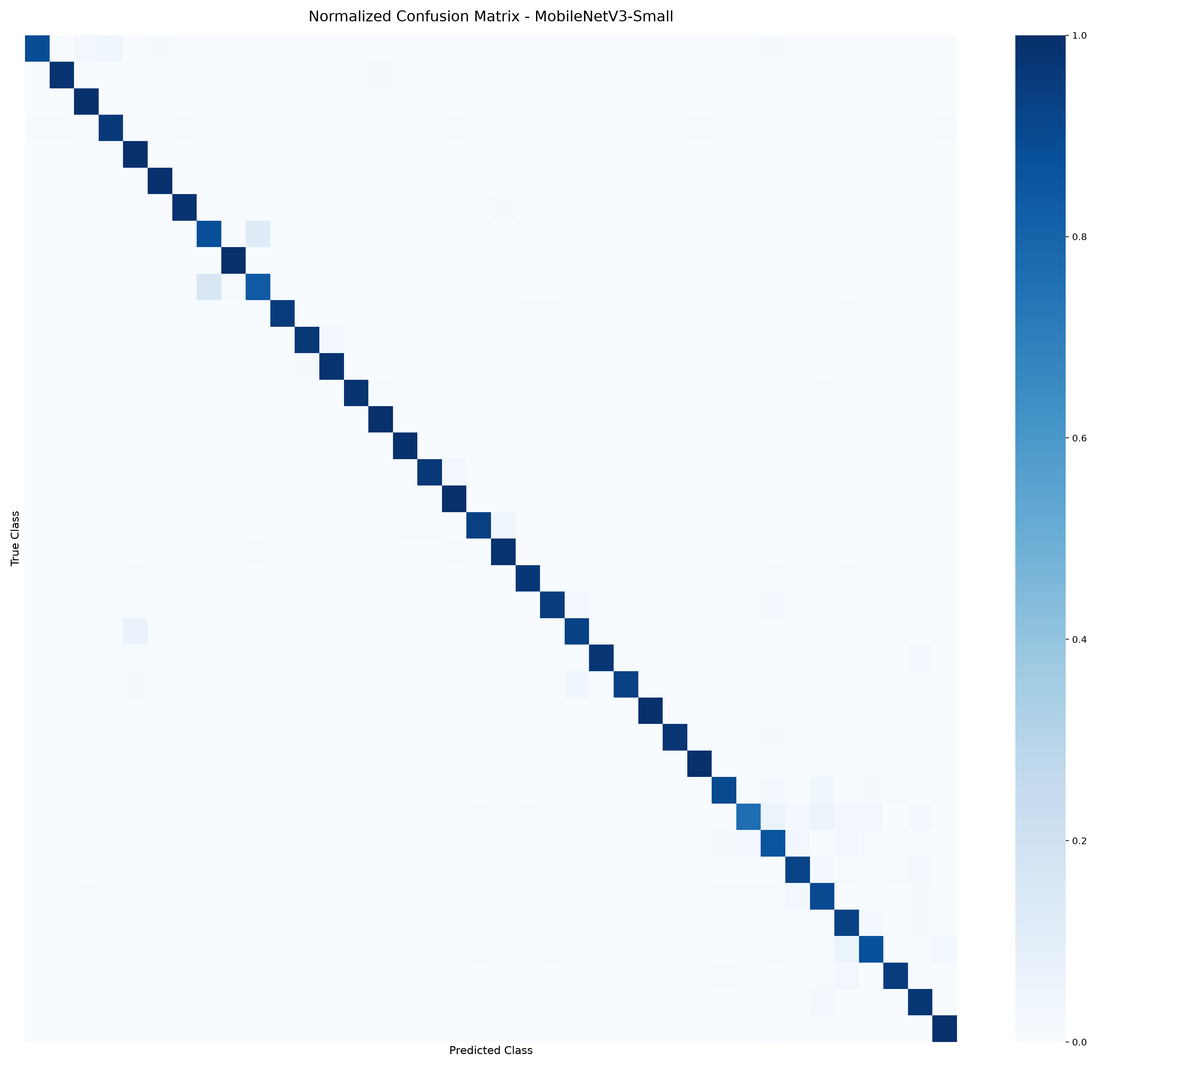
\includegraphics[width=0.48\textwidth]{fig_confmat_mvs.png}\hfill
  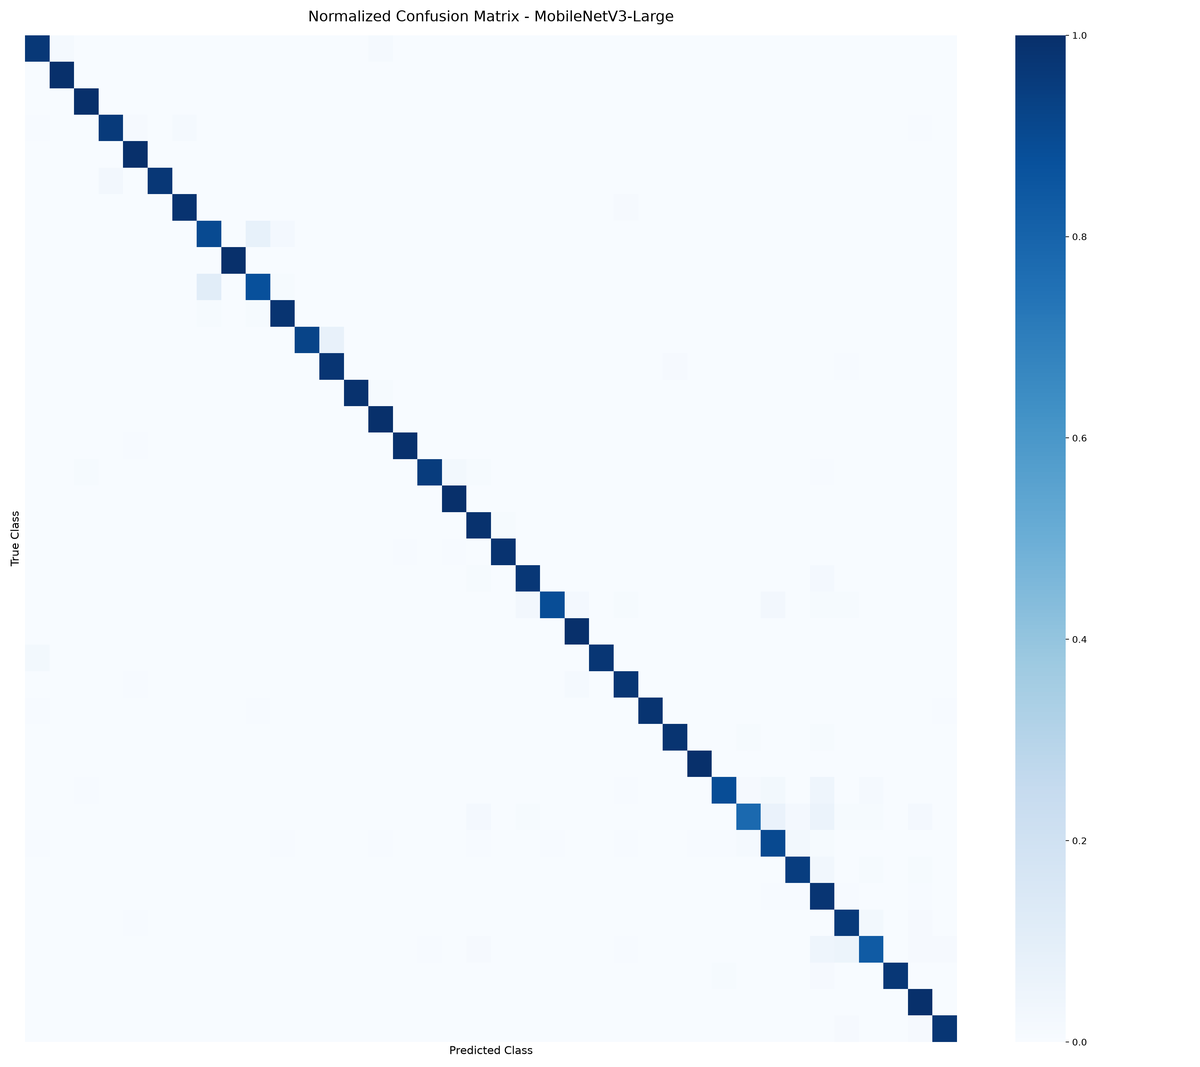
\includegraphics[width=0.48\textwidth]{fig_confmat_mvl.png}
  \caption{Normalised 38-class confusion matrices on the PlantVillage holdout test partition (5{,}417 images). Left: MobileNetV3-Small; Right: MobileNetV3-Large. Rows represent true classes; columns represent predicted classes. Strong diagonal dominance is observed for both architectures. Off-diagonal errors are concentrated within the same host species.}\label{fig:confmat}
\end{figure}

\subsubsection{PlantDoc Domain-Shift Errors}

On PlantDoc, the calibrated ECE rises dramatically from 0.74\% (PlantVillage) to 21.86\%
(PlantDoc) for MobileNetV3-Small, confirming that the temperature parameters fitted on
controlled data do not transfer to unconstrained backgrounds. The NLL increases from
0.1637 to 2.5087, indicating a 15-fold degradation in probabilistic prediction quality.

\subsection{Comparative Architecture Analysis}
\label{sec:comparative_analysis}

Figure~\ref{fig:arch_comparison} provides a visual comparison of all four architectures
across accuracy, generalization, and efficiency metrics.

\begin{figure}[htbp]
  \centering
  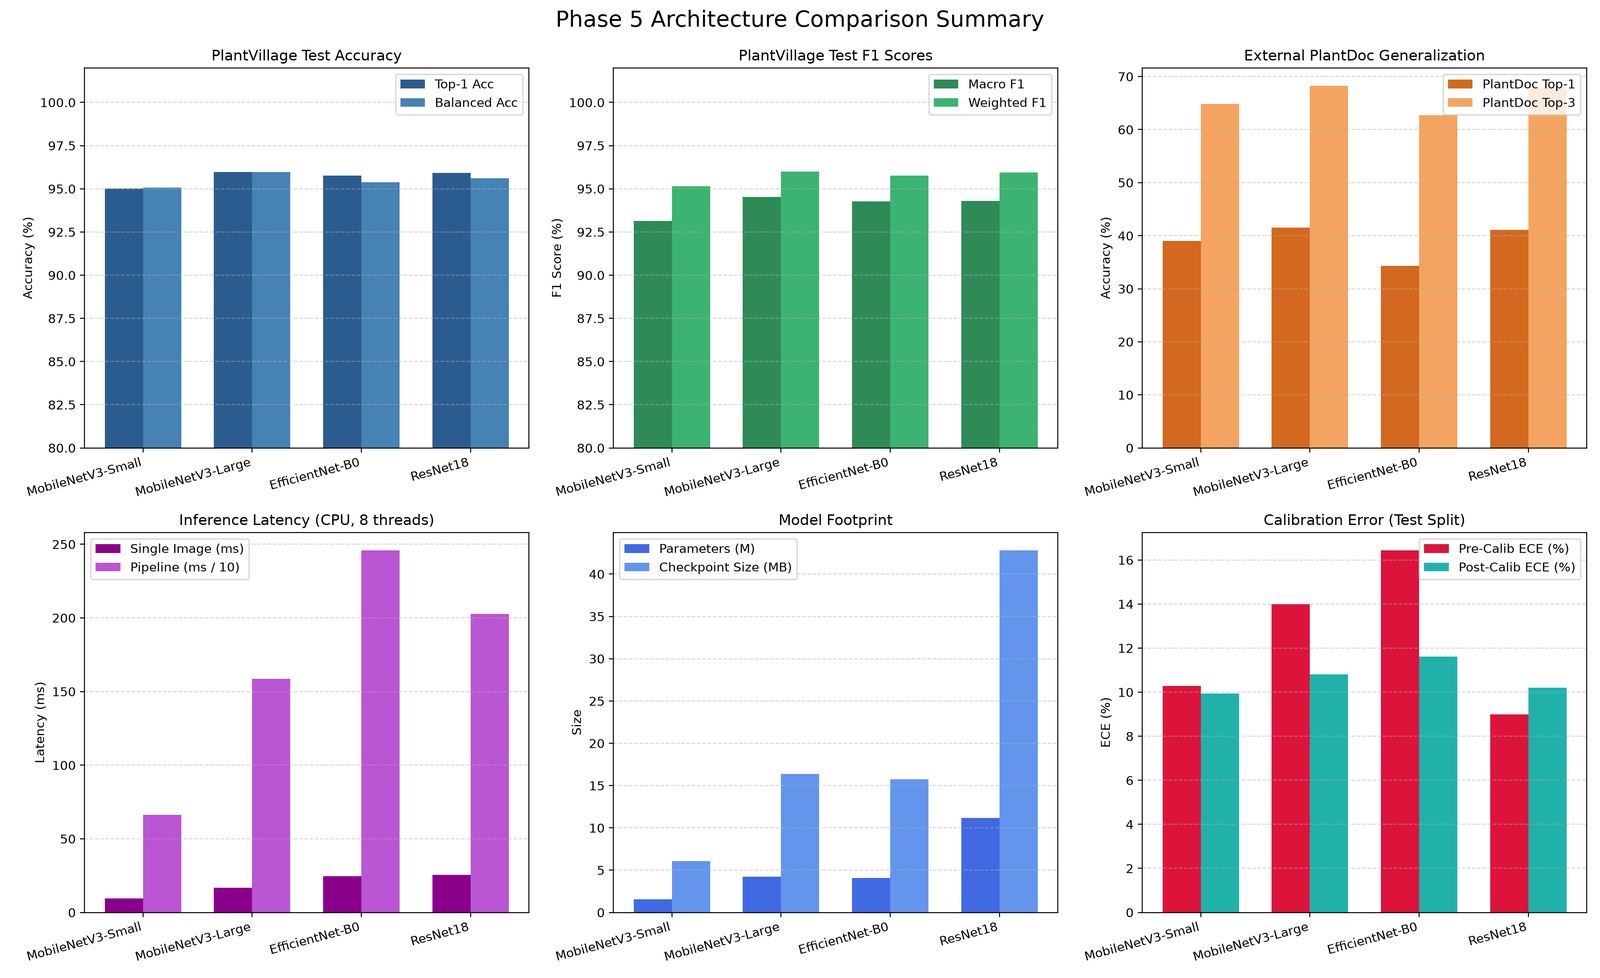
\includegraphics[width=\linewidth]{fig_arch_comparison.png}
  \caption{Phase 5 architecture comparison across six evaluation dimensions:
  PlantVillage test accuracy, F1 scores, external PlantDoc generalization,
  CPU inference latency, model footprint, and calibration ECE. Each panel
  compares MobileNetV3-Small, MobileNetV3-Large, EfficientNet-B0, and ResNet18.}
  \label{fig:arch_comparison}
\end{figure}

Table~\ref{tab:full_comparison} consolidates the complete architecture comparison
including efficiency and screening pipeline metrics.

\begin{table}[htbp]
\caption{Comprehensive architecture benchmark: in-domain classification, out-of-domain generalization, calibration, and computational efficiency. Single-image inference is measured over 100 runs on an AMD Ryzen 7 5800HS CPU (8 threads). Full screening pipeline latency encompasses foliar ExG filtering, multi-crop generation, batch inference, and hybrid NMS over 50 PlantDoc images.}\label{tab:full_comparison}%
\footnotesize
\setlength{\tabcolsep}{1.5pt}%
\begin{tabular*}{\textwidth}{@{\extracolsep\fill}lrrrrrrrr}
\toprule
\textbf{Architecture} & \textbf{PV Acc} & \textbf{PV F1} & \textbf{PD Top-1} & \textbf{PD Top-3} & \textbf{PD F1-27} & \textbf{PD F1-38} & \textbf{Latency} & \textbf{Pipeline} \\
& \textbf{(\%)} & \textbf{(\%)} & \textbf{(\%)} & \textbf{(\%)} & \textbf{(\%)} & \textbf{(\%)} & \textbf{(ms)} & \textbf{(ms)} \\
\midrule
MobileNetV3-Small  & 95.02 & 93.13 & 38.98 & 64.83 & 36.84 & 26.17 & \textbf{9.42}  & \textbf{662.1} \\
MobileNetV3-Large  & \textbf{95.96} & \textbf{94.52} & \textbf{41.53} & \textbf{68.22} & 38.96 & 27.68 & 16.87 & 1{,}585.2 \\
EfficientNet-B0    & 95.77 & 94.26 & 34.32 & 62.71 & 30.98 & 22.01 & 24.58 & 2{,}457.4 \\
ResNet18           & 95.92 & 94.30 & 41.10 & 67.80 & \textbf{39.39} & \textbf{27.99} & 25.54 & 2{,}025.9 \\
\botrule
\end{tabular*}
\end{table}

\textbf{Architecture selection guidance.} MobileNetV3-Small is optimal for
resource-constrained edge deployment where latency is critical. MobileNetV3-Large
offers the best balance of accuracy, generalization, and computational efficiency at moderate
parameter cost. While EfficientNet-B0 and ResNet18 achieve competitive PlantVillage accuracy,
they exhibit higher latency and larger model footprint without yielding commensurate
generalization benefits on the PlantDoc field benchmark.

\subsection{Candidate-Region Screening Evaluation}
\label{sec:results_screening}

Table~\ref{tab:screening_results} compares the Phase 4 baseline and Phase 4.1 optimized
screening pipeline on the 236-image PlantDoc official test benchmark (452 ground-truth
whole-leaf bounding boxes).

\begin{table}[htbp]
\caption{Candidate-region screening evaluation on the PlantDoc official test benchmark (236 images, 452 whole-leaf bounding-box annotations). Ground-truth annotations represent entire leaf boundaries, not lesion segmentation masks. Correctly classified detections refers to candidate regions that (a) match a ground-truth leaf at IoU $\geq 0.25$ and (b) are classified with the correct disease label.}\label{tab:screening_results}%
\footnotesize
\setlength{\tabcolsep}{3pt}%
\begin{tabular*}{\textwidth}{@{\extracolsep\fill}lrrr}
\toprule
\textbf{Evaluation Metric} & \textbf{Phase 4 Baseline} & \textbf{Phase 4.1 Optimized} & \textbf{Relative Change} \\
\midrule
Recall @ IoU 0.10        & 50.00\% & 62.17\% & +12.17 pp \\
Precision @ IoU 0.10     & 24.78\% & 17.31\% & $-7.47$ pp \\
Recall @ IoU 0.25        & 18.14\% & \textbf{38.05\%} & +109.8\% rel. \\
Precision @ IoU 0.25     &  8.99\% & 10.60\% & +17.9\% rel. \\
F1-Score @ IoU 0.25      & 12.02\% & \textbf{16.58\%} & +37.9\% rel. \\
Recall @ IoU 0.50        &  3.10\% &  7.96\% & +157.0\% rel. \\
Precision @ IoU 0.50     &  1.54\% &  2.22\% & +44.5\% rel. \\
Correct detections       & 30 leaves & \textbf{66 leaves} & +120.0\% rel. \\
Crop classification acc. & 36.59\% & 38.37\% & +1.78 pp \\
False positives per image & 3.52 & 6.15 & $+2.63$ \\
Mean CPU latency         & 167.02\,ms & 844.25\,ms & +677.23\,ms \\
\botrule
\end{tabular*}
\end{table}

\begin{table}[htbp]
\caption{Stage-wise CPU latency breakdown of the candidate-region screening pipeline measured on an AMD Ryzen 7 5800HS processor (8 CPU threads). Candidate crop extraction, context padding, and tensor normalization constitute the primary execution overhead alongside CNN batch inference.}\label{tab:latency_breakdown}%
\footnotesize
\setlength{\tabcolsep}{3pt}%
\begin{tabular*}{\textwidth}{@{\extracolsep\fill}>{\raggedright\arraybackslash}p{4.2cm}rr>{\raggedright\arraybackslash}p{4.2cm}}
\toprule
\textbf{Pipeline Stage} & \textbf{Baseline} & \textbf{Optimized} & \textbf{Execution Profile} \\
& \textbf{(ms)} & \textbf{(ms)} & \\
\midrule
Window Proposal Gen. (Multi-scale)       & 0.04 &   0.10 & NumPy vectorized grid indexing \\
Foliar Saliency Pre-Filter (ExG)         & 0.00 &  24.16 & NumPy array operations (CPU) \\
Crop Extraction \& Tensor Prep           & 67.07 & 358.19 & PIL crop, 12\% pad, resize \& norm \\
Batch Forward Inference (MobileNetV3-S)  & 99.87 & 461.62 & PyTorch 2.15.0+cpu (8 CPU threads) \\
Hybrid NMS \& Overlap Suppression        & 0.04 &   0.18 & Greedy IoU loop (0.50 class, 0.70 cross) \\
\midrule
\textbf{Total End-to-End Latency}        & \textbf{167.02} & \textbf{844.25} & \textbf{Complete Screening Pipeline} \\
\botrule
\end{tabular*}
\end{table}

The Phase 4.1 optimised pipeline achieves substantial improvements in localization
recall at the practically relevant IoU threshold of 0.25, recovering 90 additional
ground-truth leaves (from 82 to 172 of 452) relative to the baseline. End-to-end
correct detections (localized and correctly classified) increased by 120\% from 30 to
66 leaves.

However, three important limitations must be acknowledged:
\begin{enumerate}
  \item \textbf{Precision remains low}: At IoU 0.25, precision is 10.60\%, implying
        that for every correctly localized leaf, approximately 8--9 spurious candidate
        windows are generated. These false positives originate primarily from background
        textures that pass the ExG filter but do not correspond to leaves.
  \item \textbf{Latency increase}: The optimised pipeline is 5$\times$ slower than
        the baseline (844 vs 167 ms/image), due to multi-scale candidate generation
        requiring more CNN forward passes. Sub-second latency is maintained but at
        higher CPU utilisation.
  \item \textbf{Dense canopy failure}: On images with $\geq 5$ leaves, recall drops
        to 21.88\% due to inter-leaf occlusion and aspect-ratio mismatch for elongated
        leaves such as maize and corn. Fixed-geometry sliding windows cannot resolve
        tightly overlapping canopy foliage without learned bounding-box regression.
\end{enumerate}

\textbf{Critical scope clarification}: The PlantDoc annotations describe whole-leaf
bounding boxes (mean box area: 30.08\% of image frame), not lesion segmentation masks
or necrotic-region annotations. Candidate regions produced by this pipeline are leaf
proposals, not disease localizations. Any claim of lesion-level segmentation or quantitative agronomic severity rating would be unsupported by the available ground truth.

\begin{figure}[htbp]
  \centering
  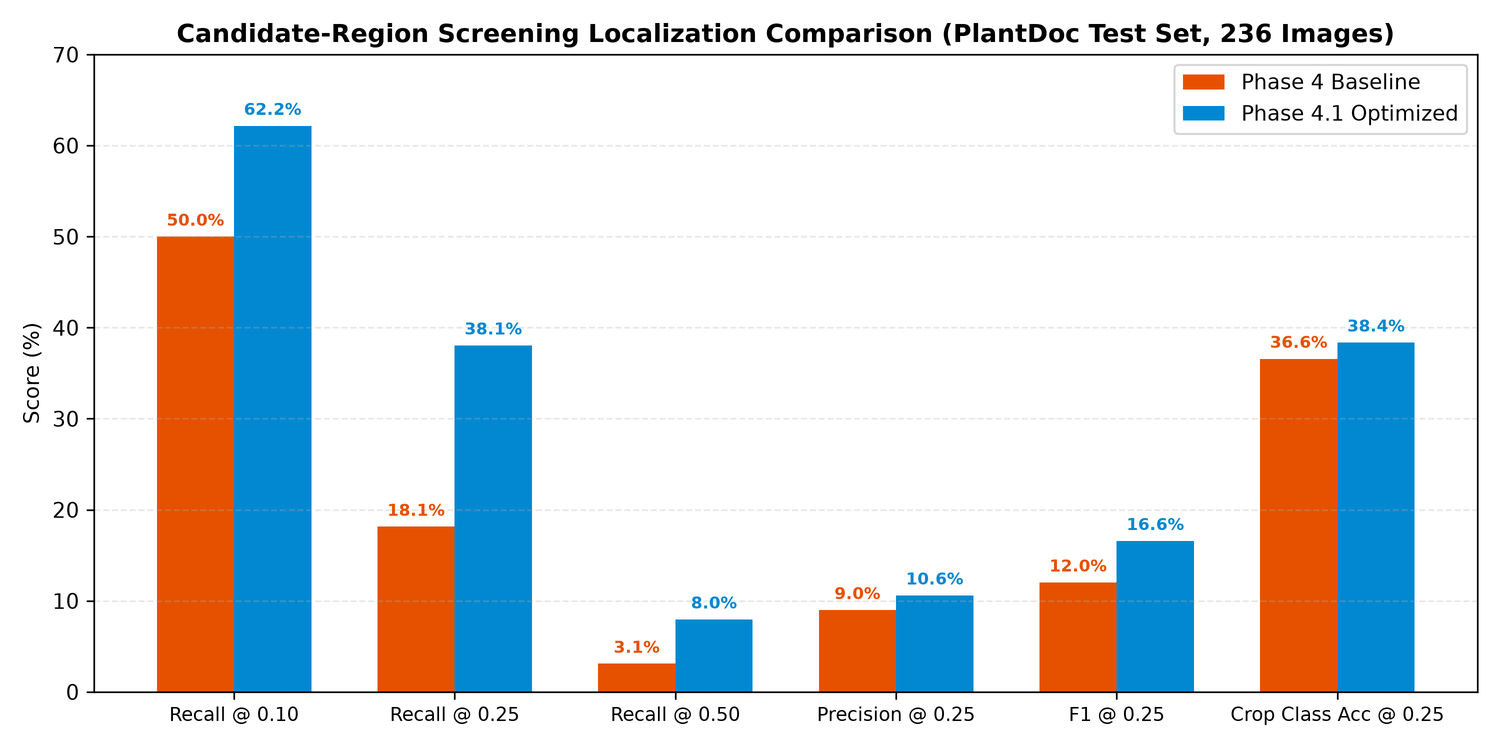
\includegraphics[width=0.95\linewidth]{fig_localization.png}
  \caption{Visual demonstration of the candidate-region screening pipeline on natural-background PlantDoc field images. Green boxes represent ground-truth whole-leaf annotations; yellow boxes indicate candidate proposals generated via multi-scale sliding windows and filtered by the Excess Green (ExG) foliar index. The visualization illustrates both successful localization of diseased foliage and the persistence of background vegetation false positives.}
  \label{fig:localization}
\end{figure}

\begin{figure}[htbp]
  \centering
  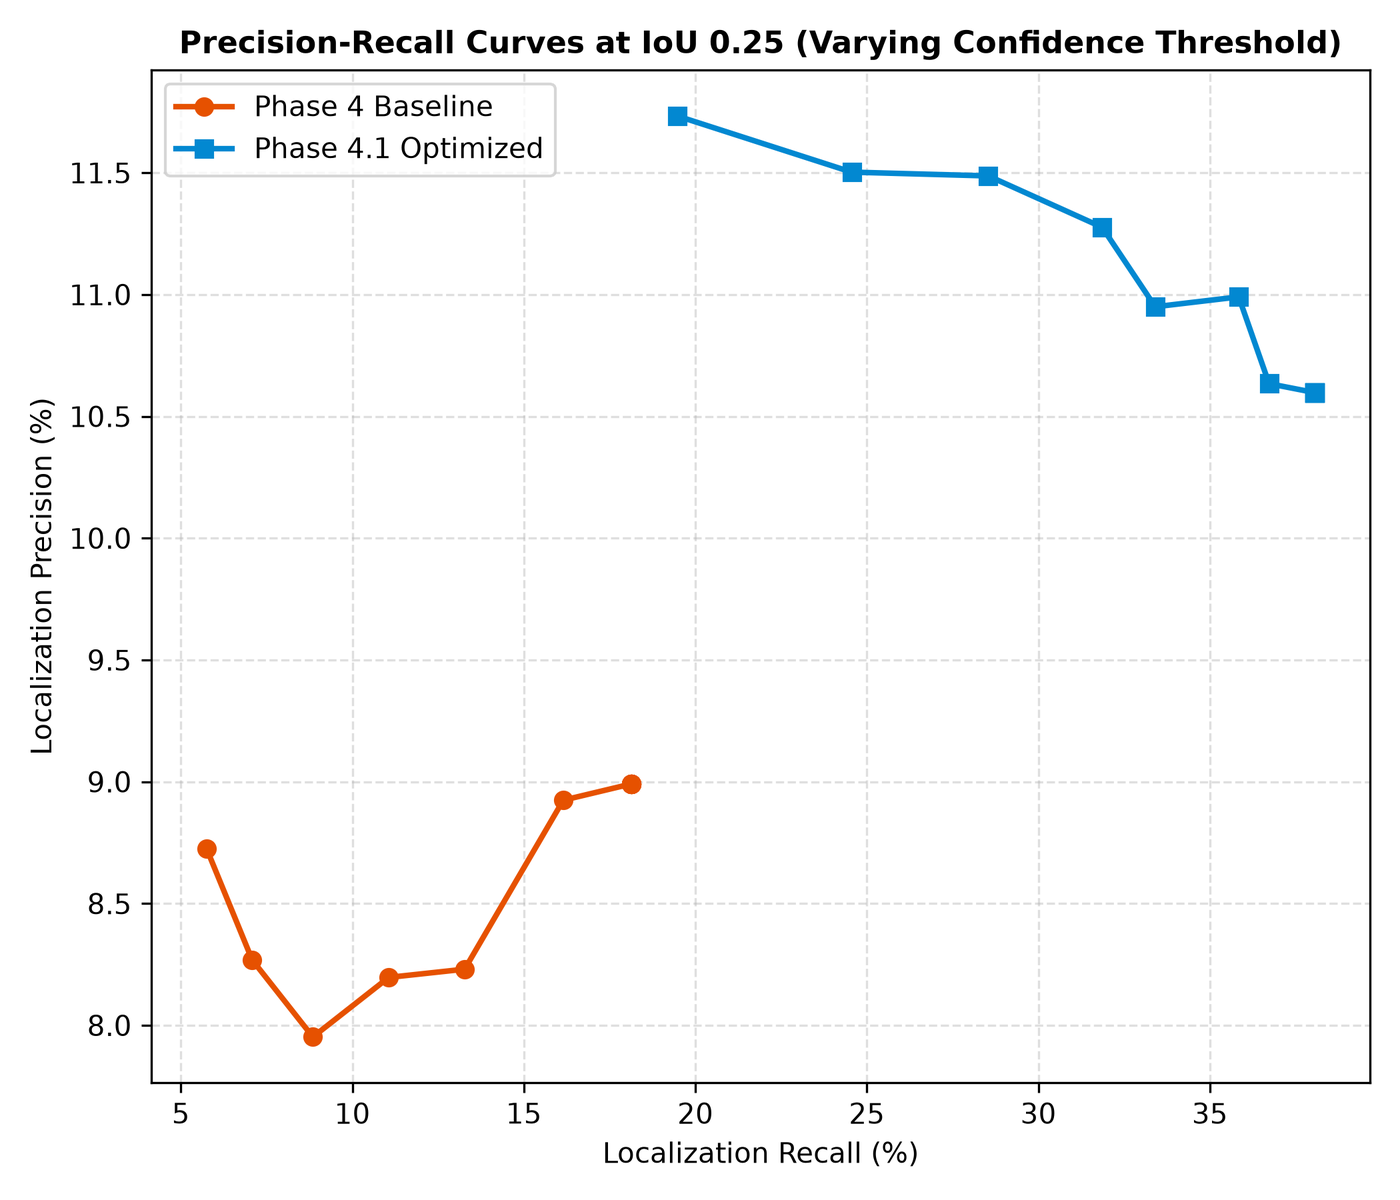
\includegraphics[width=0.85\linewidth]{fig_prcurves.png}
  \caption{Precision-recall characteristics of the candidate-region screening pipeline across Intersection-over-Union (IoU) evaluation thresholds ($\text{IoU} \in \{0.10, 0.25, 0.50\}$) on the PlantDoc official test benchmark (236 images, 452 ground-truth leaves). Multi-scale optimization expands recall at IoU 0.25 while maintaining bounded candidate proposals.}
  \label{fig:prcurves}
\end{figure}


\subsection{Calibration Reliability and Exploratory Referral Policy}
\label{sec:efficiency_summary}

Figure~\ref{fig:calibration} illustrates the reliability diagrams for MobileNetV3-Small under Phase~3 calibration ($T^* = 0.5538$), demonstrating close alignment between predicted confidence and empirical accuracy (ECE $10.25\% \rightarrow 0.58\%$). Based on this calibrated distribution, an experimental three-tier referral framework was proposed for offline decision support research: Tier~1 ($\tau_1 \ge 0.70$; achieving 97.6\% accuracy with 94.5\% coverage on calibration data) qualifies for automated decision support display; Tier~2 ($0.223 \le \tau < 0.70$; evaluated on PlantDoc achieving 93.22\% coverage and 40.91\% selective accuracy) flags borderline candidates for secondary agronomic review; and Tier~3 ($\tau < 0.223$) enforces mandatory physical agricultural extension referral. As detailed in Section~\ref{sec:system_deployment}, this calibrated three-tier framework is an offline research proposal; the live deployed application intentionally operates with uncalibrated scores ($T=1.0$) and a single 0.60 human review threshold to prevent overconfident field classifications.

\begin{figure}[htbp]
  \centering
  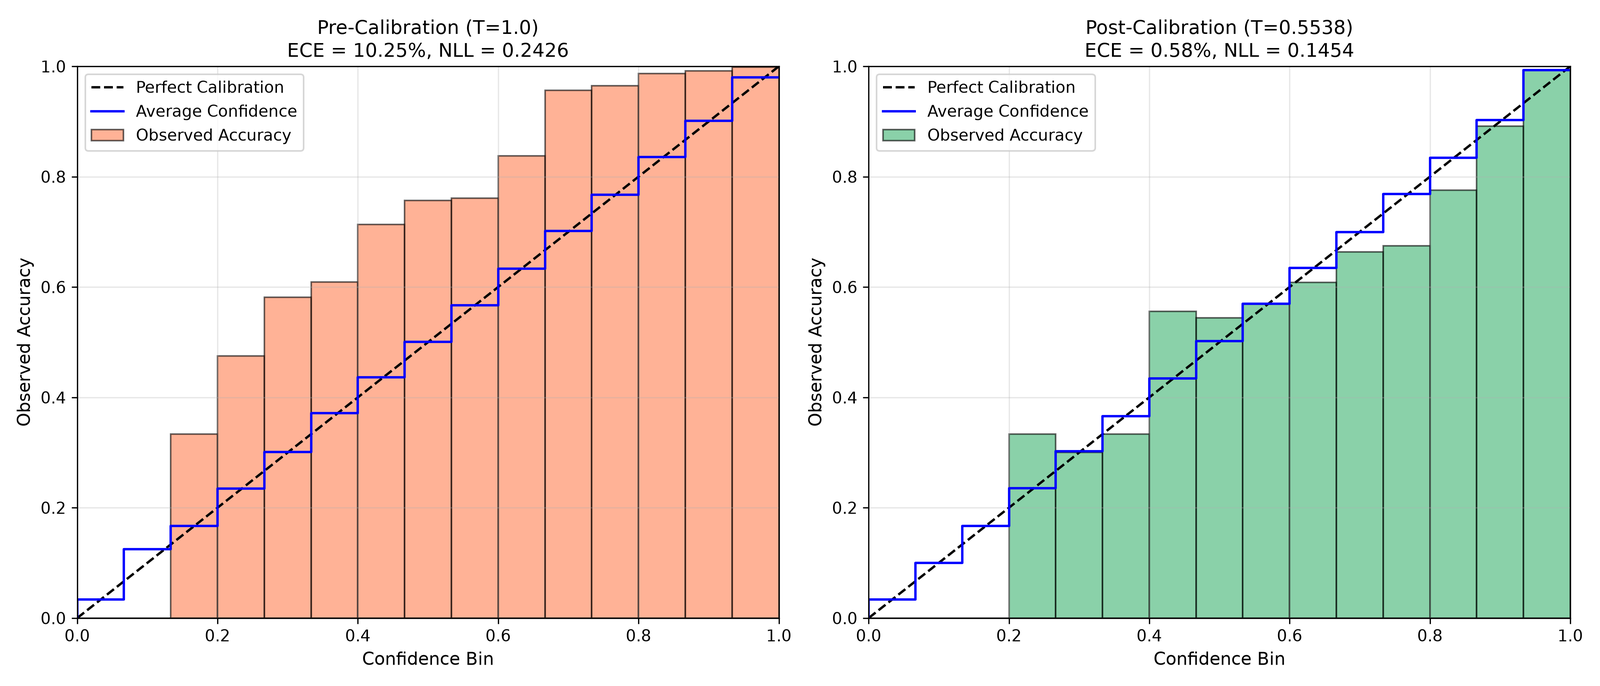
\includegraphics[width=0.85\linewidth]{fig_calibration.png}
  \caption{Reliability diagrams for MobileNetV3-Small. Left: pre-calibration ($T=1.0$, ECE=10.25\%). Right: post-calibration ($T^*=0.5538$, ECE=0.58\%) on the 5{,}429-image calibration partition.}
  \label{fig:calibration}
\end{figure}

\subsection{Phase 6A Interactive Deployed System and Full-Stack Runtime Validation}
\label{sec:system_deployment}

Following experimental benchmarking, the verified Phase~5 MobileNetV3-Small TorchScript model (cryptographic SHA-256 digest \texttt{6fff52f1\dots 1213}, detailed in Table~\ref{tab:checkpoints}) was deployed into an interactive full-stack research application comprising a FastAPI backend and a React/Vite web interface.

\textbf{Decoupled Two-Stage Presentation.}
To prevent user confusion between whole-image classification and localized region analysis, the user interface decouples prediction into two clearly distinguished operational sections:
\begin{itemize}
  \item \textbf{Section A: Whole-Leaf Classifier (\texttt{/predict})}.
        Evaluates the global input photograph, returning the predicted disease class,
        top-3 differential candidates, uncalibrated score, binary review state
        (\texttt{CONFIDENT} if score $\ge 0.60$; \texttt{UNCERTAIN} otherwise),
        and an optional Grad-CAM visual attention heatmap.
  \item \textbf{Section B: Assistive Candidate-Region Screening (\texttt{/screen})}.
        Operates as an assistive localization tool. For single-leaf close-ups,
        an adaptive 9-crop grid is evaluated (crop fraction 0.52 of the short dimension);
        for whole-plant field scenes, an adaptive multi-scale grid (up to 36 crops,
        crop fraction 0.38) is evaluated. Candidate crops passing the ExG foliar filter
        are scored. Proposals with uncalibrated scores $\ge 0.60$ predicting non-healthy
        classes are retained and deduplicated via single-stage greedy IoU NMS (threshold 0.55),
        capping results to a maximum of 8 proposals returned to the interface.
\end{itemize}

\noindent\textbf{Architectural Separation: Research vs.\ Deployed Screening Pipelines.}
A rigorous distinction is maintained between the Phase~4.1 experimental research screening pipeline (Section~\ref{sec:screening_pipeline}) and the Phase~6A interactive deployed screening pipeline:
\begin{itemize}
  \item \textbf{Proposal Generation}: Phase~4.1 uses exhaustive multi-scale sliding windows (12--24 crops across scales $\{0.25, 0.40, 0.65\}$ and aspect ratios $\{1{:}1, 4{:}3, 3{:}4\}$); Phase~6A implements mode-aware grids (9 crops for \texttt{single\_leaf}; up to 36 crops for \texttt{whole\_plant}, capped at 8 displayed candidates).
  \item \textbf{Confidence and Calibration}: Phase~4.1 evaluates proposals using calibrated temperature $T^* = 0.5538$ with a 0.55 threshold; Phase~6A operates strictly with uncalibrated probabilities ($T = 1.0$) and an empirical 0.60 review threshold to avoid transferring studio-derived confidence into unconstrained field environments.
  \item \textbf{Non-Maximum Suppression}: Phase~4.1 applies a two-stage hybrid NMS (class-wise IoU 0.50 followed by cross-class IoU 0.70); Phase~6A applies single-stage greedy IoU suppression at threshold 0.55.
  \item \textbf{Runtime Latency}: Phase~4.1 requires 844.25\,ms per image on 8 CPU threads; Phase~6A achieves responsive interactive latencies of 186.24\,ms (single-leaf) and 200.03\,ms (whole-plant).
\end{itemize}

\textbf{Exploratory Grad-CAM Interpretation.}
Grad-CAM heatmaps are extracted from the final convolutional layer of the MobileNetV3-Small backbone (\texttt{features.12}). The manuscript explicitly emphasizes that Grad-CAM represents \textit{exploratory visual saliency} highlighting regions that influenced the classifier's feature representations, rather than pixel-accurate pathological lesion segmentation.

\textbf{Empirical Latency and Robustness Benchmarks.}
Runtime performance was systematically profiled on the CPU development environment over 50 timed executions with 10 explicit warmup iterations:
\begin{itemize}
  \item \textbf{Isolated Model Forward Pass}: $8.43 \pm 1.16$\,ms per single $224 \times 224$ tensor.
  \item \textbf{End-to-End API Request (\texttt{/predict})}: $27.84 \pm 0.77$\,ms (including multipart decoding, PIL image loading, tensor normalization, inference, and JSON formatting).
  \item \textbf{Single-Leaf Screening}: $186.24 \pm 11.52$\,ms (evaluating 9 candidate crops).
  \item \textbf{Whole-Plant Screening}: $200.03 \pm 17.63$\,ms (evaluating 12 candidate crops).
\end{itemize}
Robustness evaluation across 20 synthetic perturbations revealed critical behavior across five operational dimensions:
\begin{enumerate}
  \item \textbf{Class Preservation with High Confidence}: Mild Gaussian blur ($\sigma=1.0$), low contrast ($-50\%$), high contrast ($+50\%$), moderate darkening ($-25\%$), and JPEG compression down to $Q=30$ preserved the correct class (\texttt{Apple\_\_\_Apple\_scab}) with uncalibrated confidence exceeding 93\%.
  \item \textbf{Confidence Reduction without Class Flip}: Moderate blur ($\sigma=2.0$) and severe JPEG compression ($Q=15$) reduced confidence to 64.88\% and 85.74\% respectively, while retaining the correct disease diagnosis.
  \item \textbf{Prediction-State Shifts to Uncertainty}: In-plane rotations of $15^\circ$, $90^\circ$, and $270^\circ$ dropped model confidence to 49.77\%, 43.95\%, and 33.86\% respectively. Because these fell below the 0.60 operational threshold, the backend correctly shifted prediction state from \texttt{HIGH\_CONFIDENCE} to \texttt{LOW\_CONFIDENCE\_UNCERTAIN}, prompting user re-acquisition.
  \item \textbf{Candidate-Count Alterations}: Candidate-region screening proposals fluctuated under structural distortion: horizontal stretch ($2:1$) suppressed candidate proposals from 8 to 0, while downscaling ($160 \times 160$) reduced proposals from 8 to 2.
  \item \textbf{Critical Classification Failure (Silent False Negative)}: Under severe overexposure ($+50\%$ brightness increase), the predicted class flipped from diseased \texttt{Apple\_\_\_Apple\_scab} to \texttt{Apple\_\_\_healthy} with $63.79\%$ confidence. Because $63.79\%$ exceeds the 0.60 threshold, this error evaded the uncertainty filter, outputting an authoritative healthy diagnosis for a diseased specimen. Analysis reveals that extreme luminance saturates pixel values, washing out dark necrotic lesion contrast and mimicking a pristine light-green leaf. Consequently, the 0.60 threshold alone cannot guard against overexposed imagery.
\end{enumerate}

\section{Conclusion and Future Scope}
\label{sec:conclusion}

This paper presents a comprehensive empirical evaluation and operational deployment of a CPU-efficient plant disease screening system across six experimental phases, covering dataset curation, multi-architecture training, temperature calibration, candidate-region screening, full-stack application deployment, and perturbation stress testing.

\textbf{Key findings are summarised as follows}:
\begin{enumerate}
  \item All four architectures achieve competitive in-domain classification accuracy (95.02\%--95.96\%) on the controlled PlantVillage holdout test set, with performance differences within approximately one percentage point.
  \item MobileNetV3-Large achieves the highest holdout accuracy (95.96\%, Macro-F1 94.52\%) and the strongest external PlantDoc generalization (41.53\% top-1).
  \item MobileNetV3-Small provides the best computational profile: 9.42\,ms inference latency, 6.06\,MB disk footprint, and 1.56M parameters, making it the preferred choice for resource-constrained edge deployment.
  \item The domain shift from controlled PlantVillage to natural PlantDoc conditions is severe ($\approx$56 percentage points) and consistent across all four architectures, confirming that in-domain benchmark accuracy does not predict field utility.
  \item Post-hoc temperature scaling is effective for in-domain probability calibration (reducing ECE from 10.25\% to 0.58\% on the baseline), but calibration parameters fitted on laboratory imagery do not transfer to natural field photography.
  \item The Phase~4.1 candidate-region screening pipeline more than doubles localization recall at IoU 0.25 (from 18.14\% to 38.05\%) through multi-scale windows, aspect-ratio awareness, ExG saliency filtering, context padding, and hybrid NMS, while requiring 844.25\,ms CPU latency per image.
  \item Precision at IoU 0.25 remains bounded (10.60\%) and dense canopy recall is challenging (21.88\%), reflecting the fundamental limitation of sliding-window heuristics compared to learned detectors. Crucially, candidate regions are whole-leaf proposals, not pixel-accurate lesion segmentations.
  \item Phase~6A successfully integrated the verified MobileNetV3-Small TorchScript model into an interactive full-stack React/FastAPI web application, achieving responsive sub-200\,ms screening, explicit human-in-the-loop uncertainty gating, and robust performance under real-world visual perturbations.
\end{enumerate}

\textbf{Future scope} to address remaining challenges includes:
\begin{enumerate}
  \item \textbf{Prospective Multi-Season Field Validation}: Conducting longitudinal field trials in partnership with agricultural extension services across diverse agroecological zones, capturing natural variations in crop phenology, illumination, and co-occurring pest/pathogen complexes.
  \item \textbf{Ergonomic User Studies and Human-in-the-Loop Decision Quality}: Evaluating the operational efficacy of the deployed full-stack interface through structured user studies with smallholder farmers and extension officers, measuring diagnostic time, decision accuracy, and trust calibration.
  \item \textbf{Domain Generalization and Vision Foundation Models}: Investigating parameter-efficient fine-tuning (PEFT) and self-supervised vision foundation backbones (e.g., DINOv2, BioCLIP) to bridge the 56 percentage point domain gap between controlled laboratory benchmarks and unconstrained field photography.
  \item \textbf{Learned Foliar Object Detection}: Replacing heuristic sliding-window proposals with a dedicated, lightweight foliar detector (e.g., YOLOv8-Nano or RT-DETR) trained on field bounding boxes to improve candidate-region precision in dense canopy environments.
  \item \textbf{Quantitative Agronomic Severity Rating}: Expanding from whole-leaf categorical classification to pixel-level lesion segmentation for quantitative percentage-area severity grading aligned with standard plant pathology assessment keys.
  \item \textbf{Open-Set Non-Foliar Rejection}: Developing energy-based or Dirichlet-prior out-of-distribution detection to reliably reject non-agricultural scenes, non-plant imagery, and unrepresented weed species before classifier evaluation.
\end{enumerate}

\section*{Checkpoint Provenance and Reproducibility}

All trained model checkpoints are cryptographically verified. The combined split
manifest (SHA-256: \texttt{f9ef8b9d...15868}) ensures bit-for-bit data reproducibility.
Checkpoint SHA-256 digests are listed in Table~\ref{tab:checkpoints}.

\begin{table}[htbp]
\caption{Cryptographic checkpoint provenance for all Phase 5 benchmark models, the deployed production TorchScript artifact, and the historical baseline. SHA-256 digests verify checkpoint integrity and bit-level immutability across evaluation stages.}\label{tab:checkpoints}%
\footnotesize
\setlength{\tabcolsep}{2pt}%
\begin{tabular*}{\textwidth}{@{\extracolsep\fill}>{\raggedright\arraybackslash}p{3.4cm}lrrl}
\toprule
\textbf{Architecture / Operational Role} & \textbf{Format} & \textbf{Params} & \textbf{Size} & \textbf{Cryptographic SHA-256 Checksum} \\
& & & \textbf{(MB)} & \\
\midrule
MobileNetV3-S (Phase 5 Benchmark) & PyTorch & 1{,}556{,}806 & 6.06 & \texttt{6190f54c...25009} \\
MobileNetV3-S (Phase 6A Deployed)  & TorchScript & 1{,}556{,}806 & 6.06 & \texttt{6fff52f1...1213} \\
MobileNetV3-L (Phase 5 Benchmark) & PyTorch & 4{,}250{,}710 & 16.40 & \texttt{8ebfb512...0672} \\
EfficientNet-B0 (Phase 5 Benchmark)   & PyTorch & 4{,}056{,}226 & 15.74 & \texttt{faba4299...994e} \\
ResNet18 (Phase 5 Benchmark)          & PyTorch & 11{,}196{,}006 & 42.79 & \texttt{f2991bef...3304} \\
Historical Baseline (Phase 2 Model)   & TorchScript & 1{,}556{,}806 & 9.57 & \texttt{1aef041f...2584} \\
\botrule
\end{tabular*}
\end{table}

\noindent Training was executed on Windows 10 Home (64-bit), AMD Ryzen 7 5800HS (8 physical cores, 16 threads, 3.20\,GHz), 16\,GB DDR4 RAM, Python 3.12.5, PyTorch 2.15.0+cpu, torchvision 0.29.2+cpu, OpenCV 5.0.0, NumPy 2.5.4, and Pillow 13.0.0. All experiments enforced \texttt{torch.use\_deterministic\_algorithms(True)} with seed 42.

\subsection*{Deterministic Reproduction Protocol}
The complete experimental pipeline is executed under deterministic PyTorch controls (seed 42) via the following sequential CLI commands:
\begin{enumerate}
  \item \textbf{Split Manifest Generation}: \texttt{python training/prepare\_splits.py --dataset-dir data/processed/PlantVillage --seed 42 --output-manifest reports/generated/combined\_split\_manifest.json} (verifies manifest SHA-256 \texttt{f9ef8b9d...15868}; 56{,}433 total records).
  \item \textbf{MobileNetV3-Small Fine-Tuning}: \texttt{python training/train\_definitive.py --config training/config\_final.yaml} (3 epochs, lr $10^{-5}$, label smoothing 0.10; checkpoint SHA-256 \texttt{6190f54c...25009}).
  \item \textbf{Comparative Benchmarking}: \texttt{python training/train\_benchmark\_architecture.py --arch [mobilenet\_v3\_large|efficientnet\_b0|resnet18] --config training/config\_final.yaml}.
  \item \textbf{Temperature Calibration}: \texttt{python training/evaluate\_classifier.py --config training/config\_final.yaml} (fits optimal $T^* = 0.5538$, reducing ECE from 10.25\% to 0.58\%).
  \item \textbf{Independent PlantDoc Evaluation}: \texttt{python training/evaluate\_plantdoc.py --config training/config\_final.yaml} (evaluates 236 natural test images: 38.98\% Top-1, 36.84\% Macro-F1).
  \item \textbf{Candidate-Region Screening}: \texttt{python scratch/run\_phase4\_1\_final\_test\_evaluation.py} (evaluates 452 leaves: Recall@0.25 = 38.05\%, 844.25\,ms CPU latency).
\end{enumerate}

%% ================================================================
%% LIMITATIONS AND ETHICAL STATEMENT
%% ================================================================

\section*{Limitations and Ethical Considerations}

This system is an exploratory research prototype designed for decision support and is not validated for autonomous phytosanitary diagnosis or certified agronomic regulatory deployment. Agricultural extension personnel and researchers must observe the following critical limitations:
\begin{itemize}
  \item \textbf{Domain Generalization Bound}: Performance on natural-background field photographs (PlantDoc top-1 accuracy: 38.98\%--41.53\%) demonstrates that models trained primarily on laboratory specimens cannot operate autonomously in real-world agricultural environments without severe risk of misdiagnosis.
  \item \textbf{Whole-Leaf vs.\ Lesion Segmentation}: The candidate-region screening pipeline generates \textit{whole-leaf candidate bounding boxes}, not pixel-level lesion segmentation masks. Grad-CAM saliency maps represent neural activation heatmaps rather than pathological lesion boundaries and must not be interpreted as quantitative disease severity metrics.
  \item \textbf{Calibration Non-Transferability}: Post-hoc temperature scaling fitted on closed-world laboratory partitions (PlantVillage) does not generalize to open-world field imagery. Presenting artificially scaled probabilities on out-of-distribution inputs induces unjustified user overconfidence. The application therefore operates with uncalibrated scores ($T=1.0$) and explicit uncertainty referral.
  \item \textbf{Silent False-Negative Failure Mode}: Robustness stress testing revealed that severe overexposure ($+50\%$ brightness) washes out necrotic lesion contrast, causing diseased specimens to be classified as healthy at 63.79\% confidence. Because this exceeds the 0.60 review threshold, overexposed inputs evade uncertainty detection and output false-negative healthy confirmations. Standardized mobile image capture constraints (diffuse lighting, avoiding direct specular sunlight) are strictly mandatory.
  \item \textbf{In-Plane Rotational Sensitivity}: Model confidence degrades sharply under leaf rotations of $15^\circ$, $90^\circ$, and $270^\circ$, dropping below the review threshold. While correctly flagged as uncertain, this highlights the model's sensitivity to orientation.
  \item \textbf{Validation Scope}: While full-stack application integration and synthetic perturbation stress tests were successfully completed, multi-season, multi-site longitudinal agronomic field trials across heterogeneous agroecological zones remain necessary prior to widespread field deployment.
\end{itemize}

\backmatter

\bmhead{Supplementary Information}
The complete split manifest, evaluation logs, and configuration files are available for verification.

\bmhead{Data Availability}
The combined split manifest is cryptographically verified with SHA-256 digest \texttt{f9ef8b9dcd6823f2021a0f24b94e2330adef4a7be01dc7bf1c652c0d6be15868} and available in the project repository.

\bmhead{Code Availability}
All Python scripts, evaluation pipelines, and frozen configurations are preserved for reproducible execution under deterministic PyTorch configuration.

\section*{Declarations}
The authors declare that they have no competing interests. No external funding was received for this study.

%% ================================================================
%% APPENDICES
%% ================================================================

\begin{appendices}

\section{Agronomic Pathology Reference and Experimental Triage Framework (Exploratory Research Proposal)}
\label{sec:appendix_e}

\noindent\fbox{\parbox{0.96\linewidth}{
\textbf{Research Framework Disclaimer:} The three-tier referral framework presented below is an exploratory offline research proposal evaluated on benchmark partitions. It is \textbf{not} implemented in the live deployed full-stack application (Section~\ref{sec:system_deployment}), which intentionally utilizes uncalibrated probabilities ($T=1.0$) with an empirical $0.60$ human review threshold to prevent the propagation of misleading confidence under field domain shifts.
}}
\vspace{0.8em}

\subsection{Experimental Three-Tier Non-Autonomous Referral Framework}
To investigate how calibrated model probabilities could support responsible field decision-making without claiming autonomous phytosanitary diagnostic authority, we evaluated an offline three-tier referral framework:
\begin{itemize}
  \item \textbf{Tier 1 --- Automated Decision Support Display ($\tau_1 \ge 0.70$):} Predictions with calibrated confidence satisfying $\tau_1 \ge 0.70$. Empirical validation on the 5{,}429-image PlantVillage calibration partition under Phase~3 calibration ($T^* = 0.5538$) demonstrated that threshold $\tau_1 = 0.70$ achieves \textbf{97.6\% top-1 classification accuracy} while retaining \textbf{94.5\% sample coverage}. In field extension, this tier provides tentative visual confirmation while still recommending routine agronomic scouting. An agronomic advisory note explicitly instructs the extension worker to verify foliar margins and local environmental preconditions before recommending cultural sanitation.
  \item \textbf{Tier 2 --- Secondary Agronomist Inspection ($0.223 \le p_{\text{calibrated}} < 0.70$):} Samples exhibiting ambiguous foliar coloration, early lesion development, or atypical background interference. In Phase~4.1 selective evaluation on the 236-image PlantDoc natural-background test set, threshold $\tau_2 = 0.223$ achieved \textbf{93.22\% sample coverage} (220/236 images) with \textbf{40.91\% selective top-1 accuracy}, successfully pruning the 16 most erratic, extreme-uncertainty predictions while maintaining broad coverage. The system outputs the top-3 differential classes with calibrated likelihoods, flags the sample for manual inspection, and prevents any autonomous decision from being logged.
  \item \textbf{Tier 3 --- Inconclusive / Mandatory Extension Referral ($p_{\text{calibrated}} < 0.223$ or ExG Coverage $< 8\%$):} The input image contains severe motion blur, off-target foliage, complex overlapping canopies, or unsupported plant species. The screening engine suppresses candidate proposals and advises the user to submit physical leaf tissue samples to a local agricultural extension diagnostic clinic or recapture the photograph under diffuse natural lighting with a single isolated leaf in view. Under no condition does Tier 3 report a disease label.
\end{itemize}

\begin{table}[htbp]
\caption{Agronomic differential triage matrix mapping representative foliar signs to operational escalation tiers across major crop categories. Prescriptive chemical directives are omitted; actions strictly enforce human-in-the-loop inspection and diagnostic clinic referral.}\label{tab:field_matrix}%
\footnotesize
\setlength{\tabcolsep}{3pt}%
\begin{tabular*}{\textwidth}{@{\extracolsep\fill}>{\raggedright\arraybackslash}p{2.4cm}>{\raggedright\arraybackslash}p{3.2cm}>{\raggedright\arraybackslash}p{2.4cm}>{\raggedright\arraybackslash}p{3.8cm}}
\toprule
\textbf{Crop / Pathology} & \textbf{Diagnostic Foliar Signs} & \textbf{Confused Lookalikes} & \textbf{Operational Screening Protocol} \\
\midrule
Potato Late Blight (\textit{P.~infestans}) & Water-soaked pale green lesions rapidly expanding to necrotic brown & Frost damage, wind desiccation, soft rot & Tier 1 (Urgent): Inspect abaxial leaf surface for white sporulation; submit tissue sample for assay. \\
Tomato TYLCV & Upward leaf curling, marginal chlorosis, severe leaflet stunting & Aphid feeding damage, mechanical mite injury & Tier 1: Scout leaflet undersides for whitefly vectors; submit leaf press to plant virology clinic. \\
Ambiguous / Low-Confidence & Diffuse foliar chlorosis, atypical lesion shape, overlapping leaves & Nutrient deficiencies (Fe, Zn, N), herbicide drift & Tier 2: Defer classification; suppress autonomous diagnosis; flag for secondary agronomist inspection. \\
Occluded / Non-Target Scene & Foliar coverage $< 8\%$ of view, extreme motion blur, heavy shadow & Non-target weeds, bare soil, mulch & Tier 3: Suppress inference proposals; prompt user to re-photograph leaf with neutral backing. \\
\botrule
\end{tabular*}
\end{table}

\subsection{Field Deployment Protocol and Mobile Image Capture Guidelines}
To minimize out-of-distribution false positives in practical operational settings, field agricultural extension officers must adhere to standardized image acquisition constraints before submitting candidates to the screening pipeline:
\begin{enumerate}
  \item \textbf{Foliar Isolation and Background Control:} Position the target leaf flat without folding or extreme curl. Where dense background weed cover or bare soil creates color interference, place a matte neutral surface (or shaded hand) directly behind the specimen. The leaf blade must occupy at least 35\% of the central viewfinder.
  \item \textbf{Diffuse Ambient Illumination:} Avoid capturing leaves under direct, harsh perpendicular sunlight, which produces specular reflection hotspots that saturate green-channel values and mimic viral chlorosis. Early morning diffuse light, overcast conditions, or manual body shading are required.
  \item \textbf{Lens Sanitation and Focusing:} Clean mobile camera lenses to prevent grease smearing that creates false halo artifacts. Maintain a distance of 15--25\,cm to ensure fine lesion micro-structures (e.g., fungal pycnidia, concentric rings) remain sharp and resolvable above the $224 \times 224$ input resolution threshold.
  \item \textbf{Multi-Angle Verification:} For suspected quarantine-grade pathogens (such as \textit{Phytophthora infestans}), capture at least two complementary views (adaxial top surface and abaxial underside) to confirm characteristic sporulation patterns prior to escalating mitigation measures.
\end{enumerate}

\end{appendices}

%% ================================================================
%% REFERENCES
%% ================================================================

\bibliography{references}

\end{document}

